\documentclass[11pt,a4paper]{article}

% Packages
\usepackage[utf8]{inputenc}
\usepackage[T1]{fontenc}
% \usepackage[french]{babel}  % Décommenter si babel fonctionne sur votre système
\usepackage{amsmath,amssymb}
\usepackage{bm}              % Pour \bm{} (bold math)
\usepackage{graphicx}
\usepackage{booktabs}
\usepackage{siunitx}
\usepackage{caption}
\usepackage{subcaption}
\usepackage{hyperref}
\usepackage[margin=2.5cm]{geometry}
\usepackage{float}
\usepackage[table]{xcolor}
\usepackage{comment}         % Pour \begin{comment}...\end{comment}
\usepackage{tcolorbox}       % Pour les boîtes colorées
\usepackage{mdframed}        % Pour les cadres
\usepackage{tikz}            % Pour les figures TikZ
\usetikzlibrary{arrows.meta, patterns, decorations.pathreplacing, calc, positioning, shapes.geometric}
\usepackage{listings}          
\usepackage{enumitem}          
\usepackage{inconsolata}          

% Définition des couleurs
\definecolor{brass}{RGB}{181, 166, 66}
\definecolor{tungsten}{RGB}{100, 100, 120}
\definecolor{beryllium}{RGB}{200, 220, 200}
\definecolor{aluminum}{RGB}{180, 180, 195}
\definecolor{water}{RGB}{100, 150, 220}
\definecolor{air}{RGB}{230, 240, 255}
\definecolor{steel}{RGB}{160, 160, 170}
\definecolor{Carnelian}{rgb}{0.7,0.11,0.11}
\definecolor{MyGreen}{rgb}{0.0,0.5,0.0}
\definecolor{MyGreen2}{rgb}{0.0,0.42,0.24}

\definecolor{dose1}{RGB}{255, 107, 107}
\definecolor{dose2}{RGB}{255, 160, 122}
\definecolor{dose3}{RGB}{255, 215, 0}
\definecolor{dose4}{RGB}{144, 238, 144}
\definecolor{dose5}{RGB}{135, 206, 235}
\definecolor{header}{RGB}{70, 130, 180}
\definecolor{lightgray}{RGB}{245, 245, 245}

\definecolor{graphite}{RGB}{44,62,80}
\definecolor{brass}{RGB}{212,160,23}
\definecolor{comptonblue}{RGB}{41,128,185}
\definecolor{photored}{RGB}{231,76,60}
\definecolor{codebg}{RGB}{248,248,248}

\definecolor{codegreen}{RGB}{40,140,60}
\definecolor{codegray}{RGB}{100,100,100}
\definecolor{codeblue}{RGB}{30,90,180}
\definecolor{addgreen}{RGB}{230,255,230}
\definecolor{modblue}{RGB}{230,240,255}
\definecolor{inox}{RGB}{220,232,255}


% ---- Listings ----
\lstdefinestyle{cpp}{
  language=C++,
  backgroundcolor=\color{codebg},
  basicstyle=\scriptsize\ttfamily,
  keywordstyle=\color{blue}\bfseries,
  commentstyle=\color{codegreen}\itshape,
  stringstyle=\color{gray},
  breaklines=true,
  frame=single,
  rulecolor=\color{gray!30},
  numbers=left,
  numberstyle=\tiny\color{gray},
  numbersep=5pt,
  tabsize=4,
  showstringspaces=false,
  morekeywords={G4bool,G4int,G4double,G4String,G4ThreeVector,MyTrackInfo,
                G4VUserTrackInformation,G4Step,G4Track,G4VProcess,
                G4LogicalVolume,G4AnalysisManager,G4AutoLock},
}

\lstdefinestyle{root}{
  language=C++,
  backgroundcolor=\color{codebg},
  basicstyle=\scriptsize\ttfamily,
  keywordstyle=\color{blue}\bfseries,
  frame=single,
  rulecolor=\color{gray!30},
  showstringspaces=false,
}

% Configuration siunitx
\sisetup{
    locale = FR,
    separate-uncertainty = true,
    per-mode = symbol
}

\title{%
  \vspace{-1.5cm}
  {\Large\textsc{Proposition de configuration}}\\[0.3cm]
  {\LARGE\bfseries Collimateur conique concentrateur Compton\\en graphite}\\[0.3cm]
  {\large\itshape Remplacement du syst\`eme Al\,+\,Laiton par un
  c\^one en carbone pour la focalisation de rayons X}
}
\author{%
  Application : tube Amptek MiniX (\SIrange{1}{50}{\kilo\electronvolt}, c\^one 60$^\circ$)
}
\date{\today}

\begin{document}

\maketitle
\newpage



%==============================================================================
\normalsize
\noindent \begin{mdframed}[backgroundcolor=orange!20]
\section{\Large \color{blue} \textbf{Motivation et probl\'ematique}\color{black}}
\end{mdframed}
\footnotesize
%==============================================================================

\noindent Le syst\`eme de collimation actuel (tube aluminium + tube laiton, bore cylindrique $\varnothing$\,\SI{3}{\milli\metre}) ne transmet que \color{blue}\SI{0,78}{\percent}\color{black} \; des photons primaires (run de r\'ef\'erence, \color{blue}\num{5000000}\color{black}~\'ev\'enements).\par 
\medskip
\noindent Les \color{blue}\SI{99,2}{\percent}\color{black} \; restants sont absorb\'es par effet photo\'electrique, principalement dans le laiton (\SI{60,5}{\percent}) et l'aluminium (\SI{33}{\percent}).\par

\begin{tcolorbox}[colback=white, colframe=blue, title=Objectif, fonttitle=\bfseries]
\noindent Transformer le syst\`eme de collimation en \color{blue}\textbf{concentrateur}\color{black}, capable de rediriger les photons \`a grand angle vers l'axe du faisceau, m\^eme au prix d'une l\'eg\`ere perte d'\'energie.\par 
\noindent Le porte-collimateur en inox\,304 est impos\'e et ne peut \^etre modifi\'e.
\end{tcolorbox}
\medskip

\begin{tcolorbox}[colback=white, colframe=blue, title=Id\'ee, fonttitle=\bfseries]
\noindent Exploiter la \color{blue}\textbf{diffusion Compton}\color{black} \; dans un mat\'eriau de bas num\'ero atomique $Z$ comme m\'ecanisme de redirection, en rempla\c{c}ant les tubes m\'etalliques par un c\^one unique en \color{blue}\textbf{graphite}\color{black} \; (carbone, $Z = 6$).\par 
\end{tcolorbox}

%==============================================================================
\normalsize
\noindent \begin{mdframed}[backgroundcolor=orange!20]
\section{\Large \color{blue} \textbf{Fondements physiques}\color{black}}
\end{mdframed}
\footnotesize
%==============================================================================

%===============================================================================
\normalsize
\noindent \begin{mdframed}[backgroundcolor=orange!20]
\subsection{\color{blue}\textbf{Cin\'ematique de la diffusion Compton}\color{black}}
\end{mdframed}
\footnotesize
%===============================================================================
\medskip

\noindent La diffusion Compton est la collision d'un photon avec un \'electron quasi-libre. L'\'energie du photon diffus\'e est donn\'ee par~:\par

\begin{equation*}
\bm{E'} \;=\; \frac{\bm{E}}{\bm{1} + \dfrac{\bm{E}}{\bm{m_e} \bm{c^2}}\,(\bm{1} - \cos\bm{\theta})}
\end{equation*}

\noindent o\`u $\bm{E}$ est l'\'energie incidente, $\bm{\theta}$ l'angle de diffusion et $\bm{m_e} \bm{c^2} = \SI{511}{\kilo\electronvolt}$. \color{blue}\textbf{\`A basse \'energie}\color{black} ($\bm{E} \ll \bm{m_e }\bm{c^2}$), on se trouve dans le \color{blue}\textbf{r\'egime Thomson}\color{black}~: la \color{blue}\textbf{perte d'\'energie est n\'egligeable}\color{black}.\par
\medskip
\noindent Le tableau suivant quantifie la perte d'\'energie pour le spectre du MiniX~:\par

\begin{table}[H]
\centering
\captionsetup{labelformat=empty}
\caption{\footnotesize \textit{Perte d'\'energie Compton $\bm{\Delta E} / \bm{E}$ (\%) pour diff\'erents angles et \'energies.}}
\begin{tabular}{@{}r S[table-format=1.1] S[table-format=1.1]
                    S[table-format=1.1] S[table-format=2.1]@{}}
\toprule
\footnotesize {$\bm{E}$ (keV)} &\footnotesize  {$\bm{\theta} = \bm{30^\circ}$} &\footnotesize  {$\bm{\theta} = \bm{60^\circ}$}
            &\footnotesize  {$\bm{\theta} = \bm{90^\circ}$} &\footnotesize  {$\bm{\theta} = \bm{180^\circ}$} \\
\midrule
\footnotesize 5  &\footnotesize  0.1 &\footnotesize  0.5 &\footnotesize  1.0 &\footnotesize  1.9 \\
\footnotesize 10 &\footnotesize  0.3 &\footnotesize  1.0 &\footnotesize  1.9 &\footnotesize  3.8 \\
\footnotesize 20 &\footnotesize  0.5 &\footnotesize  1.9 &\footnotesize  3.8 &\footnotesize  7.3 \\
\footnotesize 50 &\footnotesize  1.3 &\footnotesize  4.7 &\footnotesize  8.9 &\footnotesize  16.4 \\
\bottomrule
\end{tabular}
\end{table}

\begin{tcolorbox}[colback=white, colframe=blue, title=Point cl\'e, fonttitle=\bfseries]
\noindent \`a \SI{10}{\kilo\electronvolt}, m\^eme une r\'etrodiffusion compl\`ete ($\theta = 180^\circ$) ne co\^ute que \SI{3,8}{\percent} d'\'energie. Le Compton fonctionne ici comme une \textbf{r\'eflexion quasi-\'elastique}
\end{tcolorbox}

\begin{figure}[H]
\centering
\includegraphics[width=\textwidth]{Figures/fig_compton_kinematics.png}
\captionsetup{labelformat=empty}
\caption{\footnotesize \textit{\textbf{(a)}~Perte d'\'energie relative $\bm{\Delta E} / \bm{E}$ en fonction de l'angle de diffusion pour plusieurs \'energies incidentes. \`A \SI{10}{\kilo\electronvolt}, $\bm{\Delta E} < \SI{2}{\percent}$ pour $\bm{\theta} < \bm{90^\circ}$. \textbf{(b)}~Section efficace diff\'erentielle de Klein-Nishina (normalis\'ee). \`A basse \'energie la distribution est quasi-isotrope (limite de Thomson), ce qui signifie qu'environ 50\% des diffusions se font dans l'h\'emisph\`ere avant.}}
\end{figure}

%===============================================================================
\normalsize
\noindent \begin{mdframed}[backgroundcolor=orange!20]
\subsection{\color{blue}\textbf{Distribution angulaire~: la formule de Klein-Nishina}\color{black}}
\end{mdframed}
\footnotesize
%===============================================================================
\medskip

\noindent La section efficace diff\'erentielle est donn\'ee par~:

\begin{equation*}
\frac{\bm{\mathrm{d}}\bm{\sigma}}{\bm{\mathrm{d}}\bm{\Omega}} = \frac{\bm{r_e^2}}{\bm{2}}\,\bm{P}(\bm{\theta})^2 \left[ \bm{P}(\bm{\theta}) + \frac{\bm{1}}{\bm{P}(\bm{\theta})} - \sin^2\bm{\theta} \right]
\quad\text{avec}\quad \bm{P}(\bm{\theta}) = \frac{\bm{1}}{\bm{1} + \bm{\alpha}\,(\bm{1} - \cos\bm{\theta})}
\end{equation*}

\noindent o\`u $\bm{\alpha} = \bm{E} / (\bm{m_e} \bm{c^2})$ et $\bm{r_e} = \SI{2,818e-13}{\centi\metre}$. Comme le montre la figure precedante, \`a nos \'energies ($\bm{\alpha} < \bm{0,1}$) la distribution est quasi-isotrope. Cela signifie que $\sim$\textbf{50\% des interactions Compton} produiront un photon diffus\'e dans l'h\'emisph\`ere avant, exploitable pour la concentration.

\medskip

\begin{tcolorbox}[colback=white, colframe=blue, title=R\'esum\'e physique, fonttitle=\bfseries]
\noindent Entre \SIrange{5}{50}{\kilo\electronvolt}, la diffusion Compton est \textbf{(i)}~quasi-\'elastique ($\bm{\Delta E}/\bm{E} < \bm{4}\%$) et \textbf{(ii)}~quasi-isotrope ($\sim$50\% forward). C'est un m\'ecanisme id\'eal pour \textbf{rediriger} des photons sans les d\'etruire\par 
\end{tcolorbox}

%==============================================================================
\normalsize
\noindent \begin{mdframed}[backgroundcolor=orange!20]
\section{\Large \color{blue} \textbf{Choix du mat\'eriau}\color{black}}
\end{mdframed}
\footnotesize
%==============================================================================

%===============================================================================
\normalsize
\noindent \begin{mdframed}[backgroundcolor=orange!20]
\subsection{\color{blue}\textbf{Crit\`eres de s\'election}\color{black}}
\end{mdframed}
\footnotesize
%===============================================================================
\medskip

\noindent Pour que la diffusion Compton domine l'absorption photo\'electrique, il faut~:\par

\begin{enumerate}
\item $\bm{Z}$ \textbf{bas} --- $\bm{\sigma_{\text{photo}}} \propto \bm{Z}^{4\text{--}5}$ tandis que $\bm{\sigma_{\text{Compton}}} \propto \bm{Z}$. Passer de $\bm{Z} = \bm{29}$ (laiton) \`a $\bm{Z} = \bm{6}$ (carbone) r\'eduit le rapport photo/Compton d'un facteur $\sim \bm{(29/6)^4} \approx \bm{550}$.
\item \textbf{Densit\'e suffisante} --- pour obtenir une probabilit\'e d'interaction significative dans $\sim$\SI{2}{\milli\metre} de paroi.
\end{enumerate}

%===============================================================================
\normalsize
\noindent \begin{mdframed}[backgroundcolor=orange!20]
\subsection{\color{blue}\textbf{Comparaison des mat\'eriaux candidats}\color{black}}
\end{mdframed}
\footnotesize
%===============================================================================
\medskip

\begin{figure}[H]
\centering
\includegraphics[width=\textwidth]{Figures/fig_materiaux_comparaison.png}
\captionsetup{labelformat=empty}
\caption{\footnotesize  \textit{\textbf{(a)}~Fraction de l'att\'enuation lin\'eique due au Compton. Le graphite et le b\'eryllium atteignent les fractions les plus \'elev\'ees au-dessus de \SI{10}{\kilo\electronvolt}. Le laiton reste domin\'e par le photo\'electrique sur tout le spectre. \textbf{(b)}~Probabilit\'e de diffusion Compton dans \SI{2,1}{\milli\metre} de paroi. Le graphite offre la probabilit\'e la plus \'elev\'ee en valeur absolue gr\^ace \`a sa densit\'e ($\bm{\rho} = \SI{2,26}{\gram\per\centi\metre\cubed}$).}}
\end{figure}
\begin{table}[H]
\centering
\captionsetup{labelformat=empty}
\caption{\footnotesize Propri\'et\'es des mat\'eriaux candidats pour le c\^one Compton (\SI{2,1}{\milli\metre} de paroi, $E = \SI{10}{\kilo\electronvolt}$).}
\small
\begin{tabular}{@{}l c c c c l@{}}
\toprule
\footnotesize \textbf{Mat\'eriau}&\footnotesize $Z_{\text{eff}}$&\footnotesize $\rho$ (g/cm$^3$)&\footnotesize $P_{\text{Compt}}$&\footnotesize $P_{\text{photo}}$&\footnotesize \textbf{Remarques} \\
\midrule
\rowcolor{graphite!10}
\footnotesize \textbf{Graphite (C)}&\footnotesize \textbf{6}&\footnotesize \textbf{2,26}&\footnotesize \textbf{6,0\%}&\footnotesize 32\%&\footnotesize \textbf{Meilleur compromis}\\
\footnotesize B\'eryllium (Be)&\footnotesize 4&\footnotesize 1,85&\footnotesize 4,2\%&\footnotesize 0,4\%&\footnotesize Toxique, co\^uteux \\
\footnotesize PMMA&\footnotesize 6,5&\footnotesize 1,19&\footnotesize 3,4\%&\footnotesize 14\%&\footnotesize Fond \`a 160\,$^\circ$C \\
Poly\'ethyl\`ene &\footnotesize 5,5&\footnotesize 0,94&\footnotesize 2,9\%&\footnotesize 7\%&\footnotesize Trop l\'eger, mou \\
\footnotesize B$_4$C&\footnotesize 5,2 &\footnotesize 2,52&\footnotesize 4,5\%&\footnotesize 18\%& Tr\`es dur \`a usiner\\
\midrule
\footnotesize Laiton (r\'ef.)&\footnotesize 29&\footnotesize 8,73&\footnotesize $\ll 0,1$\%&\footnotesize $> 99{,}9$\%&\footnotesize  Tout est absorb\'e \\
\bottomrule
\end{tabular}
\end{table}
\medskip

\begin{tcolorbox}[colback=white, colframe=blue, title=Conclusion, fonttitle=\bfseries]
\noindent Le \textbf{graphite} (\texttt{G4\_GRAPHITE},$\bm{\rho} = \SI{2,26}{\gram\per\centi\metre\cubed}$, $\bm{Z} = \bm{6}$) est le meilleur candidat. Il combine~:
\begin{itemize}
\item le meilleur taux de Compton absolu (gr\^ace \`a sa densit\'e \'elev\'ee parmi les bas-$\bm{Z}$),
\item une suppression forte du photo\'electrique ($\bm{Z^4}$ bas),
\item une excellente tenue thermique ($> \SI{3000}{\celsius}$ sous atmosph\`ere inerte),
\item une bonne usinabilit\'e.
\end{itemize}
\end{tcolorbox}


\clearpage

%===============================================================================
\normalsize
\noindent \begin{mdframed}[backgroundcolor=orange!20]
\subsection{\color{blue}\textbf{Devenir d'un photon dans le graphite}\color{black}}
\end{mdframed}
\footnotesize
%===============================================================================
\medskip

\begin{figure}[H]
\centering
\includegraphics[width=0.6\textwidth]{Figures/fig_devenir_photons_graphite.png}
\captionsetup{labelformat=empty}
\caption{\footnotesize \textit{R\'epartition du devenir d'un photon traversant environ \SI{3}{\milli\metre} de graphite (chemin effectif pour incidence rasante dans le c\^one). \`A\SI{10}{\kilo\electronvolt}, environ 8\% subissent un Compton, 60\% sont photo-absorb\'es et 32\% traversent sans interaction. Au-del\`a de \SI{20}{\kilo\electronvolt}, le Compton devient le processus d'interaction dominant.}}
\end{figure}

%==============================================================================
\normalsize
\noindent \begin{mdframed}[backgroundcolor=orange!20]
\section{\Large \color{blue} \textbf{G\'eom\'etrie propos\'ee~: le c\^one concentrateur}\color{black}}
\end{mdframed}
\footnotesize
%==============================================================================

%===============================================================================
\normalsize
\noindent \begin{mdframed}[backgroundcolor=orange!20]
\subsection{\color{blue}\textbf{Principe de fonctionnement}\color{black}}
\end{mdframed}
\footnotesize
%===============================================================================
\medskip

\noindent L'id\'ee est de remplacer le collimateur cylindrique (Al + Laiton) par un \textbf{collimateur conique} en graphite, \'elas\'e c\^ot\'e source et r\'etr\'eci c\^ot\'e d\'etecteur. Le c\^one agit en trois zones~:

\begin{enumerate}
\item \textbf{Zone de transmission directe} ($\theta < 3{,}2^\circ$)~: les photons traversent le bore sans interaction $\longrightarrow$ faisceau primaire inchang\'e.
\item \textbf{Zone de capture Compton} ($3{,}2^\circ < \theta < 30^\circ$)~: les photons frappent la paroi interne du c\^one en graphite sous \textbf{incidence rasante}, traversant un chemin effectif de \SIrange{3}{15}{\milli\metre}. Une fraction significative subit une diffusion Compton et est redirig\'ee vers l'avant avec $> \SI{98}{\percent}$ de son \'energie.
\item \textbf{Zone d'absorption} ($\theta > 30^\circ$)~: les photons traversent le graphite (trop mince \`a l'entr\'ee) et sont absorb\'es par le porte-collimateur inox.
\end{enumerate}

\begin{figure}[H]
\centering
\includegraphics[width=1.1\textwidth]{Figures/fig_geometry_cone_compton_graphite.png}
\captionsetup{labelformat=empty}
\caption{\footnotesize \textit{Coupe longitudinale $(r,z)$ des deux configurations. \textbf{(a)}~Syst\`eme actuel~: tous les photons hors du c\^one g\'eom\'etrique \'etroit sont absorb\'es dans le laiton.\textbf{(b)}~C\^one graphite~: le bore conique intercepte les photons \`a angle interm\'ediaire, les diffuse par Compton et les redirige vers le plan de scoring.}}
\end{figure}

%===============================================================================
\normalsize
\noindent \begin{mdframed}[backgroundcolor=orange!20]
\subsection{\color{blue}\textbf{Param\`etres g\'eom\'etriques}\color{black}}
\end{mdframed}
\footnotesize
%===============================================================================
\medskip

\noindent Le c\^one s'inscrit dans le volume libre \`a l'int\'erieur du porte-collimateur ($R_{\text{int}} = \SI{3,17}{\milli\metre}$).\par 

\begin{figure}[H]
\centering
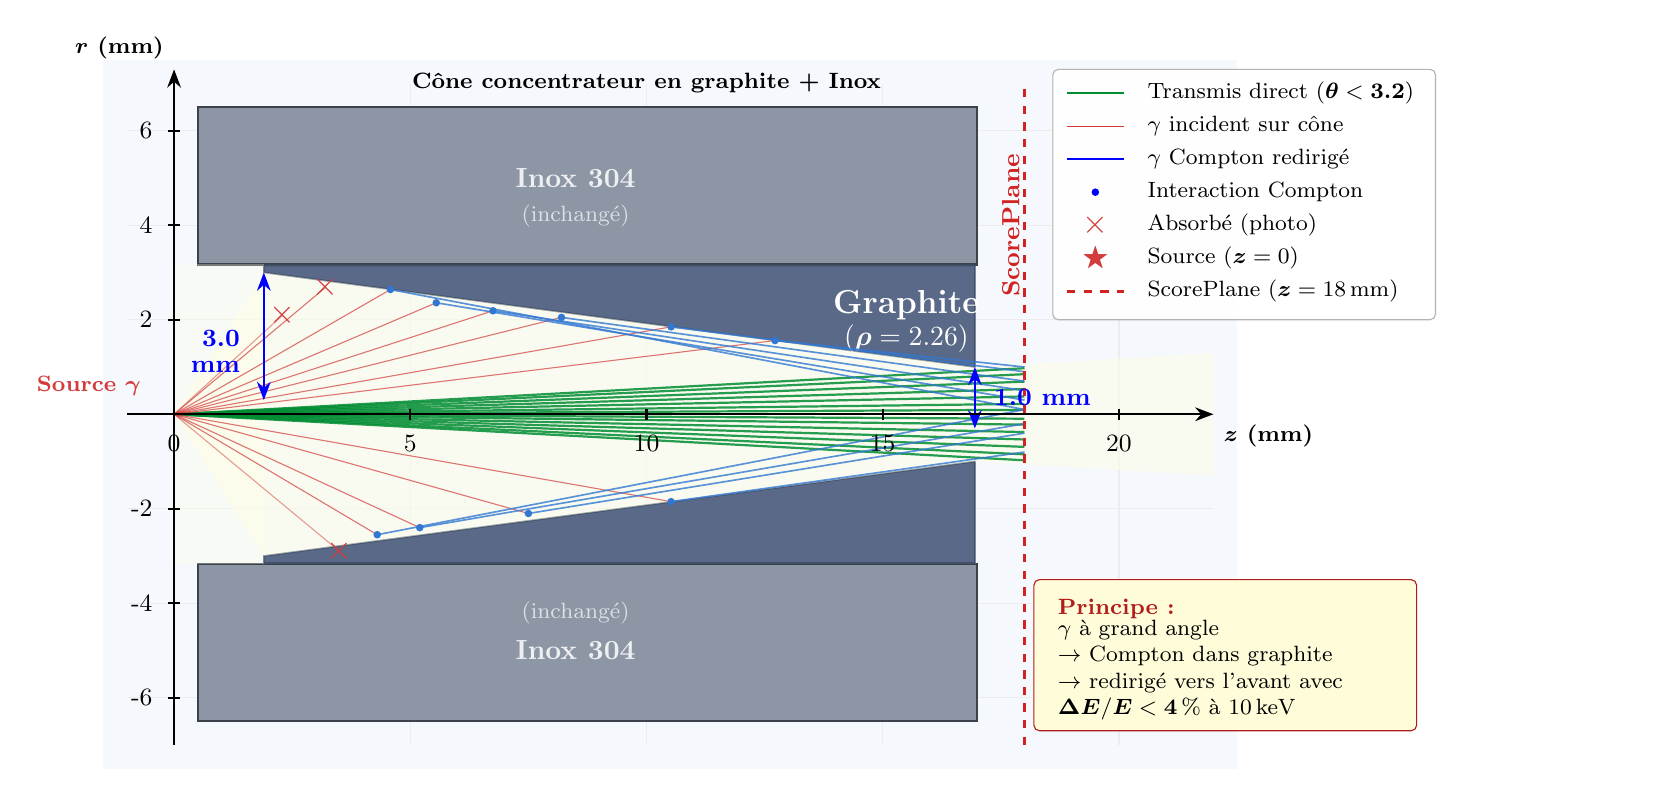
\begin{tikzpicture}[
  xscale=0.6,
  yscale=0.6,
]

% ---- Couleurs fidèles à la figure de référence ----
\definecolor{cInox}{RGB}{60,65,75}       % gris-bleu foncé pour inox
\definecolor{cInoxFill}{RGB}{140,150,165} % remplissage inox
\definecolor{cGraphite}{RGB}{65,80,105}   % bleu-gris foncé graphite
\definecolor{cGraphFill}{RGB}{90,105,135} % remplissage graphite
\definecolor{cChannel}{RGB}{255,255,230}  % jaune très pâle (canal)
\definecolor{cBg}{RGB}{245,248,252}       % fond
\definecolor{cGreen}{RGB}{0,140,50}       % vert — transmission directe
\definecolor{cRed}{RGB}{210,60,60}        % rouge — γ incident
\definecolor{cBlue}{RGB}{50,120,210}      % bleu — Compton redirigé
\definecolor{cCyan}{RGB}{0,210,220}       % cyan — annotations cotes
\definecolor{cScore}{RGB}{210,35,35}      % rouge ScorePlane

% ==================================================================
%  FOND
% ==================================================================
\fill[cBg] (-1.5,-7.5) rectangle (22.5, 7.5);

% ==================================================================
%  GRILLE LÉGÈRE (optionnel, comme fond matplotlib)
% ==================================================================
\foreach \z in {0,5,10,15,20} {
  \draw[gray!15, thin] (\z,-7) -- (\z,7);
}
\foreach \r in {-6,-4,-2,0,2,4,6} {
  \draw[gray!15, thin] (-1,\r) -- (22,\r);
}

% ==================================================================
%  INOX 304 — blocs extérieurs (porte-collimateur)
% ==================================================================
% Bloc supérieur : z=0.5..17, r=3.17..6.5
\fill[cInoxFill]
  (0.5, 3.17) rectangle (17, 6.5);
\draw[cInox, thick]
  (0.5, 3.17) -- (17, 3.17) -- (17, 6.5) -- (0.5, 6.5) -- cycle;

% Bloc inférieur
\fill[cInoxFill]
  (0.5,-6.5) rectangle (17,-3.17);
\draw[cInox, thick]
  (0.5,-6.5) -- (17,-6.5) -- (17,-3.17) -- (0.5,-3.17) -- cycle;

% Labels inox
\node[font=\normalsize\bfseries, text=white, opacity=0.85]
  at (8.5, 5.0) {Inox 304};
\node[font=\small, text=white, opacity=0.7]
  at (8.5, 4.2) {\footnotesize (inchang\'e)};
\node[font=\normalsize\bfseries, text=white, opacity=0.85]
  at (8.5,-5.0) {Inox 304};
\node[font=\small, text=white, opacity=0.7]
  at (8.5,-4.2) {\footnotesize (inchang\'e)};

% ==================================================================
%  GRAPHITE — cône concentrateur
% ==================================================================
% Géométrie du cône :
%   Face source  (z=1.90) : R_in = 3.00, R_out = 3.15
%   Face sortie  (z=16.95): R_in = 1.00, R_out = 3.15
% En coupe (z,r), le graphite est un trapèze

% Moitié supérieure (r > 0)
\fill[cGraphFill]
  (1.90, 3.15) -- (16.95, 3.15) -- (16.95, 1.00) -- (1.90, 3.00) -- cycle;
\draw[cGraphite, semithick]
  (1.90, 3.15) -- (16.95, 3.15) -- (16.95, 1.00) -- (1.90, 3.00) -- cycle;

% Moitié inférieure (r < 0)
\fill[cGraphFill]
  (1.90,-3.15) -- (16.95,-3.15) -- (16.95,-1.00) -- (1.90,-3.00) -- cycle;
\draw[cGraphite, semithick]
  (1.90,-3.15) -- (16.95,-3.15) -- (16.95,-1.00) -- (1.90,-3.00) -- cycle;

% Labels graphite
\node[font=\large\bfseries, text=white]
  at (15.5, 2.3) {Graphite};
\node[font=\normalsize, text=white]
  at (15.5, 1.6) {($\bm{\rho}=2.26$)};

% ==================================================================
%  CANAL CENTRAL — rempli en jaune pâle
% ==================================================================
\fill[cChannel, opacity=0.5]
  (0, 0) -- (1.90, 3.00) -- (16.95, 1.00)
  -- (22, 1.00*22/16.95) -- (22, -1.00*22/16.95)
  -- (16.95,-1.00) -- (1.90,-3.00) -- cycle;
% Petite zone avant le cône
\fill[cChannel, opacity=0.3]
  (0,-3.17) rectangle (1.90, 3.17);

% ==================================================================
%  TRAJECTOIRES — TRANSMISSION DIRECTE (vert, θ < 3.2°)
% ==================================================================
% Angles directs : passent à travers le canal sans toucher le cône
% Max angle pour passer : atan(1.0/16.95) ≈ 3.38°
% À z=18, r = 18*tan(θ)

% Rayons positifs
\foreach \angle in {0.3, 0.7, 1.2, 1.7, 2.2, 2.7, 3.1} {
  \pgfmathsetmacro{\rend}{18*tan(\angle)}
  \draw[cGreen, thick, opacity=0.85]
    (0,0) -- (18, \rend);
}
% Rayons négatifs (symétrique)
\foreach \angle in {-0.3, -0.7, -1.2, -1.7, -2.2, -2.7, -3.1} {
  \pgfmathsetmacro{\rend}{18*tan(\angle)}
  \draw[cGreen, thick, opacity=0.85]
    (0,0) -- (18, \rend);
}
% Rayon axial
\draw[cGreen, thick] (0,0) -- (18, 0);

% ==================================================================
%  TRAJECTOIRES — γ INCIDENT SUR CÔNE (rouge/rose)
%  puis γ COMPTON REDIRIGÉ (bleu)
% ==================================================================
% Surface intérieure du cône : r(z) = 3.0 - (2.0/15.05)*(z - 1.9)
% Rayon depuis (0,0) à angle θ : r = z*tan(θ)
% Intersection : z_hit = 3.2525 / (tan(θ) + 0.13289)

% --- Moitié supérieure (r > 0) ---
% Hit points computed:
%   θ=7°   → z=12.72, r=1.56
%   θ=10°  → z=10.52, r=1.85
%   θ=13°  → z=8.58,  r=1.98
%   θ=17°  → z=7.01,  r=2.14
%   θ=22°  → z=5.72,  r=2.31
%   θ=28°  → z=4.73,  r=2.52
%   θ=35°  → z=3.90,  r=2.73
%   θ=45°  → z=3.04,  r=3.04 (near entrance, likely absorbed)

% Hit point 1: θ≈7°, z=12.72, r=1.56
\draw[cRed, thin, opacity=0.7] (0,0) -- (12.72, 1.56);
\fill[cBlue] (12.72, 1.56) circle (0.08);
\draw[cBlue, semithick, opacity=0.8] (12.72, 1.56) -- (18, 1.0);

% Hit point 2: θ≈10°, z=10.52, r=1.85
\draw[cRed, thin, opacity=0.7] (0,0) -- (10.52, 1.85);
\fill[cBlue] (10.52, 1.85) circle (0.08);
\draw[cBlue, semithick, opacity=0.8] (10.52, 1.85) -- (18, 0.9);

% Hit point 3: θ≈14°, z=8.20, r=2.05
\draw[cRed, thin, opacity=0.7] (0,0) -- (8.20, 2.05);
\fill[cBlue] (8.20, 2.05) circle (0.08);
\draw[cBlue, semithick, opacity=0.8] (8.20, 2.05) -- (18, 0.7);

% Hit point 4: θ≈18°, z=6.75, r=2.19
\draw[cRed, thin, opacity=0.7] (0,0) -- (6.75, 2.19);
\fill[cBlue] (6.75, 2.19) circle (0.08);
\draw[cBlue, semithick, opacity=0.8] (6.75, 2.19) -- (18, 0.5);

% Hit point 5: θ≈23°, z=5.55, r=2.36
\draw[cRed, thin, opacity=0.7] (0,0) -- (5.55, 2.36);
\fill[cBlue] (5.55, 2.36) circle (0.08);
\draw[cBlue, semithick, opacity=0.8] (5.55, 2.36) -- (18, 0.3);

% Hit point 6: θ≈30°, z=4.58, r=2.64
\draw[cRed, thin, opacity=0.7] (0,0) -- (4.58, 2.64);
\fill[cBlue] (4.58, 2.64) circle (0.08);
\draw[cBlue, semithick, opacity=0.8] (4.58, 2.64) -- (18, 0.1);

% Absorbed in graphite (red X): θ≈40° → near entrance
\draw[cRed, thin, opacity=0.7] (0,0) -- (3.20, 2.68);
\node[cRed, font=\large\bfseries] at (3.20, 2.68) {$\times$};

% Absorbed (red X) near z=2.5 — photon absorbed deep in cone
\draw[cRed, thin, opacity=0.5] (0,0) -- (2.3, 2.1);
\node[cRed, font=\large\bfseries] at (2.3, 2.1) {$\times$};

% --- Moitié inférieure (r < 0) ---
% Hit point 1: z=10.52, r=-1.85
\draw[cRed, thin, opacity=0.7] (0,0) -- (10.52,-1.85);
\fill[cBlue] (10.52,-1.85) circle (0.08);
\draw[cBlue, semithick, opacity=0.8] (10.52,-1.85) -- (18,-0.8);

% Hit point 2: z=7.5, r=-2.10
\draw[cRed, thin, opacity=0.7] (0,0) -- (7.5,-2.10);
\fill[cBlue] (7.5,-2.10) circle (0.08);
\draw[cBlue, semithick, opacity=0.8] (7.5,-2.10) -- (18,-0.4);

% Hit point 3: z=5.2, r=-2.40
\draw[cRed, thin, opacity=0.7] (0,0) -- (5.2,-2.40);
\fill[cBlue] (5.2,-2.40) circle (0.08);
\draw[cBlue, semithick, opacity=0.8] (5.2,-2.40) -- (18,-0.2);

% Hit point 4: z=4.3, r=-2.55
\draw[cRed, thin, opacity=0.7] (0,0) -- (4.3,-2.55);
\fill[cBlue] (4.3,-2.55) circle (0.08);
\draw[cBlue, semithick, opacity=0.8] (4.3,-2.55) -- (18, 0.1);

% Absorbed in cone (lower)
\draw[cRed, thin, opacity=0.5] (0,0) -- (3.5,-2.90);
\node[cRed, font=\large\bfseries] at (3.5,-2.90) {$\times$};

% ==================================================================
%  SOURCE γ — étoile rouge à l'origine
% ==================================================================
%\node[cRed, font=\huge] at (0,0) {$\bigstar$};
\node[cRed, font=\footnotesize\bfseries, anchor=east] at (-0.5, 0.6) {\footnotesize Source $\bm{\gamma}$};

% ==================================================================
%  SCOREPLANE — z = 18 mm (ligne tiretée rouge)
% ==================================================================
\draw[cScore, very thick, dashed] (18,-7) -- (18, 7);
\node[cScore, font=\small\bfseries, rotate=90, anchor=south]
  at (18.1, 4) {ScorePlane};

% ==================================================================
%  ANNOTATIONS DIMENSIONNELLES (cyan)
% ==================================================================

% R = 3.0 mm (entrée) — flèche verticale
\draw[blue, thick, {Stealth}-{Stealth}]
  (1.90, 0.3) -- (1.90, 3.00);
\node[blue, font=\small\bfseries, anchor=east] at (1.6, 1.6) {\textbf{3.0}};
\node[blue, font=\small\bfseries, anchor=east] at (1.6, 1.0) {\textbf{mm}};
% Label "R=3.0mm (entrée)"
%\node[blue, font=\scriptsize, anchor=north west, text opacity=0.9]
%  at (2.1, 3.2) {$R\!=\!3.0$\,mm};
%\node[blue, font=\scriptsize, anchor=north west, text opacity=0.9]
%  at (2.1, 2.7) {(entr\'ee)};

% R = 1.0 mm (sortie) — flèche verticale
\draw[blue, thick, {Stealth}-{Stealth}]
  (16.95, -0.3) -- (16.95, 1.00);
\node[blue, font=\small\bfseries, anchor=west] at (17.15, 0.35) {\textbf{1.0 mm}};
% Label
%\node[blue, font=\scriptsize, anchor=south west, text opacity=0.9]
%  at (15.3, 1.15) {$R\!=\!1.0$\,mm};
%\node[blue, font=\scriptsize, anchor=north west, text opacity=0.9]
%  at (15.3, 1.0) {(sortie)};

% ==================================================================
%  LÉGENDE (boîte blanche, coin supérieur droit)
% ==================================================================
\begin{scope}[shift={(18.9, 5.8)}]
  \fill[white, opacity=0.92, rounded corners=2pt]
    (-0.3,-3.8) rectangle (7.8, 1.5);
  \draw[gray!60, thin, rounded corners=2pt]
    (-0.3,-3.8) rectangle (7.8, 1.5);

  % Ligne verte — transmis direct
  \draw[cGreen, thick] (0, 1.0) -- (1.2, 1.0);
  \node[font=\small, anchor=west] at (1.5, 1.0)
    {\footnotesize Transmis direct ($\bm{\theta} < \bm{3.2}°$)};

  % Ligne rouge — γ incident
  \draw[cRed, thin] (0, 0.3) -- (1.2, 0.3);
  \node[font=\footnotesize, anchor=west] at (1.5, 0.3)
    {\footnotesize $\gamma$ incident sur c\^one};

  % Ligne bleue — Compton redirigé
  \draw[blue, semithick] (0,-0.4) -- (1.2,-0.4);
  \node[font=\footnotesize, anchor=west] at (1.5,-0.4)
    {\footnotesize $\gamma$ Compton redirig\'e};

  % Point bleu — interaction Compton
  \fill[blue] (0.6,-1.1) circle (0.08);
  \node[font=\footnotesize, anchor=west] at (1.5,-1.1)
    {\footnotesize Interaction Compton};

  % Croix rouge — absorbé
  \node[cRed, font=\large\bfseries] at (0.6,-1.8) {$\times$};
  \node[font=\footnotesize, anchor=west] at (1.5,-1.8)
    {\footnotesize Absorb\'e (photo)};

  % Étoile source
  \node[cRed, font=\normalsize] at (0.6,-2.5) {$\bigstar$};
  \node[font=\footnotesize, anchor=west] at (1.5,-2.5)
    {\footnotesize Source ($\bm{z} = 0$)};

  % ScorePlane
  \draw[cScore, thick, dashed] (0,-3.2) -- (1.2,-3.2);
  \node[font=\footnotesize, anchor=west] at (1.5,-3.2)
    {\footnotesize ScorePlane ($\bm{z} = 18$\,mm)};
\end{scope}

% ==================================================================
%  BOÎTE PRINCIPE PHYSIQUE (jaune pâle, coin inférieur droit)
% ==================================================================
\begin{scope}[shift={(18.5, -4.0)}]
  \fill[yellow!15, rounded corners=2pt]
    (-0.3,-2.7) rectangle (7.8, 0.5);
  \draw[Carnelian, thin, rounded corners=2pt]
    (-0.3,-2.7) rectangle (7.8, 0.5);

    \node[font=\footnotesize\bfseries, text=Carnelian, anchor=north west]
    at (0, 0.3) {Principe :};
  \node[font=\footnotesize, anchor=north west, text width=7.2cm, align=left]
    at (0,-0.15)
    {$\gamma$ \`a grand angle\\
     $\to$ Compton dans graphite\\
     $\to$ redirig\'e vers l'avant avec\\
     $\bm{\Delta} \bm{E}/\bm{E} < \bm{4}\,\%$ \`a \SI{10}{\kilo\electronvolt}};
\end{scope}

% ==================================================================
%  AXES
% ==================================================================
\draw[->, >=Stealth, thick] (-1,0) -- (22, 0)
  node[below right, font=\footnotesize\bfseries] {$\bm{z}$ (mm)};
\draw[->, >=Stealth, thick] (0,-7) -- (0, 7.3)
  node[above left, font=\footnotesize\bfseries] {$\bm{r}$ (mm)};

% Graduations z
\foreach \z in {0, 5, 10, 15, 20} {
  \draw[thick] (\z,-0.12) -- (\z, 0.12);
  \node[below, font=\small] at (\z,-0.25) {\z};
}

% Graduations r
\foreach \r in {-6,-4,-2, 2, 4, 6} {
  \draw[thick] (-0.12,\r) -- (0.12,\r);
  \node[left, font=\small] at (-0.25,\r) {\r};
}

% ==================================================================
%  TITRE
% ==================================================================
\node[font=\footnotesize\bfseries, anchor=south]
  at (10, 6.6)
  {C\^one concentrateur en graphite + Inox};

\end{tikzpicture}
\captionsetup{labelformat=empty}
\caption{\footnotesize \textit{Coupe $(\bm{z}, \bm{r})$ du c\^one Compton en graphite + Inox~304.
Vert : transmission directe ($\bm{\theta} < \bm{3.2}°$).
Rouge : $\bm{\gamma}$ incident sur le c\^one.
Bleu : $\bm{\gamma}$ redirig\'e vers l'avant apr\`es diffusion Compton
($\bm{\Delta} \bm{E}/\bm{E} < \bm{4}\,\%$ \`a 10\,keV).
Croix : absorption photo\'electrique.}}
\end{figure}

\noindent Le tableau suivant donne les dimensions.\par

\begin{table}[H]
\centering
\captionsetup{labelformat=empty}
\caption{\footnotesize Param\`etres g\'eom\'etriques du c\^one concentrateur.}
\renewcommand{\arraystretch}{1.15}
\begin{tabular}{@{}l c l@{}}
\toprule
\footnotesize \textbf{Param\`etre} &\footnotesize  \textbf{Valeur} &\footnotesize  \textbf{Description} \\
\midrule
\multicolumn{3}{@{}l}{\footnotesize \textit{Collimateur conique (surface interne)}} \\
\footnotesize $\bm{R_{\text{in,entr\'ee}}}$&\footnotesize \SI{3,0}{\milli\metre}&\footnotesize  Rayon c\^ot\'e source (large) \\
\footnotesize $\bm{R_{\text{in,sortie}}}$  &\footnotesize \SI{1,0}{\milli\metre}&\footnotesize  Rayon c\^ot\'e d\'etecteur (\'etroit) \\
\footnotesize Demi-angle du c\^one    &\footnotesize 7,6$^\circ$&\footnotesize $\bm{\alpha} = \arctan\!\dfrac{\bm{R_{\text{in,e}}} - \bm{R_{\text{in,s}}}}{\bm{L}}$ \\[6pt]
\midrule
\multicolumn{3}{@{}l}{\footnotesize \textit{Enveloppe ext\'erieure}} \\
\footnotesize $\bm{R_{\text{ext}}}$ &\footnotesize  \SI{3,15}{\milli\metre} &\footnotesize $= \bm{R_{\text{int,inox}}} - \SI{0,02}{\milli\metre}$ (jeu) \\
\midrule
\multicolumn{3}{@{}l}{\footnotesize \textit{Dimensions axiales}} \\
\footnotesize $\bm{z_{\text{d\'ebut}}}$&\footnotesize \SI{1,90}{\milli\metre}&\footnotesize Face c\^ot\'e source \\
\footnotesize $\bm{z_{\text{fin}}}$&\footnotesize \SI{16,95}{\milli\metre}&\footnotesize Face c\^ot\'e d\'etecteur \\
Longueur               &\footnotesize  \SI{15,05}{\milli\metre}&\footnotesize\\
\midrule
\multicolumn{3}{@{}l}{\footnotesize \textit{\'Epaisseur de paroi}} \\
\footnotesize C\^ot\'e entr\'ee&\footnotesize \SI{0,15}{\milli\metre}&\footnotesize  Mince --- photons \`a grand angle traversent \\
\footnotesize C\^ot\'e sortie&\footnotesize \SI{2,15}{\milli\metre}&\footnotesize  \'Epaisse --- bonne probabilit\'e d'interaction \\
\midrule
\footnotesize Mat\'eriau Geant4&\footnotesize \texttt{G4\_GRAPHITE}&\footnotesize Carbone,$\rho = \SI{2,26}{\gram\per\centi\metre\cubed}$ \\
\bottomrule
\end{tabular}
\end{table}

% ==================================================================
%  TABLE 1 : Détail du cône Compton
% ==================================================================
\begin{table}[H]
\centering
\captionsetup{labelformat=empty}
\caption{\footnotesize \textit{\textbf{Param\`etres g\'eom\'etriques du c\^one Compton
(\texttt{G4Cons}, graphite $\bm{\rho} = 2.21$~g/cm$^3$)}}}
\medskip
{\footnotesize
\renewcommand{\arraystretch}{1.15}
\begin{tabular}{lrl}
\toprule
\footnotesize \textbf{Param\`etre} &\footnotesize \textbf{Valeur} &\footnotesize \textbf{Unit\'e} \\
\midrule
\footnotesize $\bm{R_{\mathrm{in}}^{\mathrm{entr\acute{e}e}}}$ (c\^ot\'e source, $\bm{z} = 1.90$ mm)
  &\footnotesize $3.00$ &\footnotesize mm \\
\footnotesize $\bm{R_{\mathrm{in}}^{\mathrm{sortie}}}$ (c\^ot\'e d\'etecteur, $\bm{z} = 16.95$ mm)
  &\footnotesize $1.00$ &\footnotesize mm \\
\footnotesize $\bm{R_{\mathrm{ext}}}$ (constant)
  &\footnotesize $3.15$ &\footnotesize mm \\
\footnotesize $\bm{z_{\mathrm{front}}}$
  &\footnotesize $1.90$ &\footnotesize mm \\
\footnotesize $\bm{z_{\mathrm{back}}}$
  &\footnotesize $16.95$ &\footnotesize mm \\
\footnotesize $\bm{z_{\mathrm{center}}}$
  &\footnotesize $9.425$ &\footnotesize mm \\
\footnotesize Longueur totale
  &\footnotesize $15.05$ &\footnotesize mm \\
\footnotesize Demi-longueur
  &\footnotesize $7.525$ &\footnotesize mm \\
\footnotesize Demi-angle d'ouverture $\alpha$
  &\footnotesize $7.57$ &\footnotesize deg \\
\footnotesize \'Epaisseur entr\'ee ($\bm{R_{\mathrm{ext}}} - \bm{R_{\mathrm{in}}^{\mathrm{ent}}}$)
  &\footnotesize $0.15$ &\footnotesize mm \\
\footnotesize \'Epaisseur sortie ($\bm{R_{\mathrm{ext}}} - \bm{R_{\mathrm{in}}^{\mathrm{sort}}}$)
  &\footnotesize $2.15$ &\footnotesize mm \\
\footnotesize Jeu avec porte-collimateur ($\bm{R_{\mathrm{int}}^{\mathrm{PC}}} - \bm{R_{\mathrm{ext}}}$)
  &\footnotesize $0.02$ &\footnotesize mm (nominal) \\
\midrule
\multicolumn{3}{l}{\footnotesize \textit{Angle de transmission directe maximal :}} \\[2pt]
\multicolumn{3}{c}{\footnotesize $\bm{\theta_{\max}} = \arctan\!\left(\dfrac{\bm{R_{\mathrm{in}}^{\mathrm{sort}}}}{\bm{z_{\mathrm{back}}}}\right)
                    = \arctan\!\left(\dfrac{1.00}{16.95}\right) \approx 3.38°$} \\
\bottomrule
\end{tabular}
}
\end{table}

% ==================================================================
%  TABLE 2 : Volumes principaux
% ==================================================================
\begin{table}[H]
\centering
\captionsetup{labelformat=empty}
\caption{\footnotesize \textit{\textbf{Volumes principaux de la g\'eom\'etrie (extraits de \texttt{DetectorConstruction.cc}).
Tous les composants GDML sont plac\'es \`a $(0,0,0)$ dans l'enveloppe.
La sym\'etrie cylindrique autour de l'axe~$z$ implique $R = \sqrt{x^2 + y^2}$.}}}
\medskip
{\footnotesize
\renewcommand{\arraystretch}{1.15}
\begin{tabular}{llcccc}
\toprule
\footnotesize \textbf{Composant}&\footnotesize \textbf{Mat\'eriau ($\rho$)}
&\footnotesize $\bm{z_{\min}}$&\footnotesize $\bm{z_{\max}}$
&\footnotesize $\bm{R_{\min}}$ &\footnotesize $\bm{R_{\max}}$ \\
&\footnotesize \textbf{(g/cm$^3$)}&\footnotesize \textbf{(mm)}&\footnotesize \textbf{(mm)}
&\footnotesize \textbf{(mm)} &\footnotesize \textbf{(mm)} \\
\midrule
\multicolumn{6}{l}{\footnotesize \textit{--- \textbf{Enveloppe et monde} ---}} \\
\footnotesize Monde (\texttt{G4Box})
  &\footnotesize Air&\footnotesize $-300$&\footnotesize $+300$&\multicolumn{2}{c}{\footnotesize $300\times300$~mm$^2$} \\
Enveloppe GDML (\texttt{G4Box})
  &\footnotesize Air&\footnotesize $-60$&\footnotesize $+60$&\multicolumn{2}{c}{\footnotesize $50\times50$~mm$^2$} \\[4pt]

\multicolumn{6}{l}{\textit{--- \textbf{Tube X MiniX (composants GDML, pos.\ $(0,0,0)$)} ---}} \\
Enveloppe inox
  &\footnotesize  304 (8.00) & \multicolumn{2}{c}{\footnotesize (tessell\'e)} & --- & $\sim6.5$ \\
Tube alumine
  &\footnotesize  Al$_2$O$_3$ (3.97) & \multicolumn{2}{c}{(tessell\'e)} &\footnotesize  $\sim3.8$ &\footnotesize  $\sim5.2$ \\
Vide anode/fen\^etre
  &\footnotesize  Vacuum & \multicolumn{2}{c}{\footnotesize (tessell\'e)} &\footnotesize  0 &\footnotesize  $\sim3.8$ \\
Vide cathode/anode
  &\footnotesize  Vacuum & \multicolumn{2}{c}{\footnotesize (tessell\'e)} &\footnotesize  0 &\footnotesize  $\sim3.8$ \\
\textbf{Anode tungst\`ene}
  &\footnotesize  \textbf{W (19.35)} &\footnotesize  $\mathbf{-0.001}$ &\footnotesize  $\mathbf{0.000}$
  &\footnotesize  $0$ &\footnotesize  $3.5$ \\
Fen\^etre b\'eryllium
  &\footnotesize  Be (1.848) & \multicolumn{2}{c}{\footnotesize (tessell\'e, $z\gtrsim0$)}
  &\footnotesize  0 &\footnotesize  $\sim3.5$ \\
Porte-collimateur
  &\footnotesize  304 (8.00) & \multicolumn{2}{c}{\footnotesize (tessell\'e)}
  &\footnotesize  $3.17$ &\footnotesize  $\sim5.5$ \\[4pt]

\multicolumn{6}{l}{\textit{--- \textbf{C\^one Compton ({\normalfont\texttt{G4Cons}})} ---}} \\
\textbf{C\^one graphite}
  &\footnotesize  \textbf{Graphite (2.21)}
  &\footnotesize  $\mathbf{1.90}$ &\footnotesize  $\mathbf{16.95}$
  & \multicolumn{2}{c}{} \\[4pt]

\multicolumn{6}{l}{\textit{--- \textbf{Plans de scoring} ---}} \\
ScorePlane  (\texttt{G4Box}, $1\;\mu$m)
  &\footnotesize  Air & \multicolumn{2}{c}{\footnotesize $\bm{z_c} = 18.00$}
  & \multicolumn{2}{c}{\footnotesize $50\times50$~mm$^2$} \\
ScorePlane2 (\texttt{G4Box}, 1\;mm)
  &\footnotesize  Air &\footnotesize  $27.50$ &\footnotesize  $28.50$
  & \multicolumn{2}{c}{\footnotesize $50\times50$~mm$^2$} \\
ScorePlane3 (\texttt{G4Box}, 1\;mm)
  &\footnotesize  Air &\footnotesize  $37.50$ &\footnotesize  $38.50$
  & \multicolumn{2}{c}{$50\times50$~mm$^2$} \\
ScorePlane5 (\texttt{G4Box}, 1\;mm)
  &\footnotesize  Air &\footnotesize  $69.50$ &\footnotesize  $70.50$
  & \multicolumn{2}{c}{\footnotesize $50\times50$~mm$^2$} \\[4pt]

\multicolumn{6}{l}{\textit{--- \textbf{Syst\`eme de d\'etection (couronnes d'eau + PVC)} ---}} \\
Fond PVC (\texttt{G4Tubs})
  &\footnotesize PVC (1.30)&\footnotesize $68.00$&\footnotesize $69.00$&\footnotesize $0$&\footnotesize $11.0$ \\
Paroi PVC (\texttt{G4Tubs})
  &\footnotesize PVC (1.30)&\footnotesize $65.00$&\footnotesize $68.00$&\footnotesize $10.0$&\footnotesize $11.0$ \\
Couronne~0 (\texttt{G4Tubs})
  &\footnotesize $H_2O$ (1.00)&\footnotesize $65.00$&\footnotesize $68.00$&\footnotesize $0$&\footnotesize $2.0$ \\
Couronne~1
  &\footnotesize $H_2O$ (1.00)&\footnotesize $65.00$&\footnotesize $68.00$&\footnotesize $2.0$&\footnotesize $4.0$ \\
Couronne~2
  &\footnotesize $H_2O$ (1.00)&\footnotesize $65.00$&\footnotesize $68.00$&\footnotesize $4.0$&\footnotesize $6.0$ \\
Couronne~3
  &\footnotesize $H_2O$ (1.00)&\footnotesize $65.00$&\footnotesize $68.00$&\footnotesize $6.0$&\footnotesize $8.0$ \\
Couronne~4
  &\footnotesize $H_2O$ (1.00)&\footnotesize $65.00$&\footnotesize $68.00$&\footnotesize $8.0$&\footnotesize $10.0$ \\
\bottomrule
\end{tabular}
}
\end{table}

% ==================================================================
%  TABLE 3 : Positions clés le long de z
% ==================================================================
\begin{table}[H]
\centering
\captionsetup{labelformat=empty}
\caption{\footnotesize \textit{\textbf{Rep\`eres principaux le long de l'axe~$z$, de la source au dernier plan de scoring.}}}
\medskip
{\footnotesize
\renewcommand{\arraystretch}{1.15}
\begin{tabular}{rll}
\toprule
\footnotesize $\bm{z}$ \textbf{(mm)} &\footnotesize  \textbf{Rep\`ere} &\footnotesize  \textbf{Note} \\
\midrule
\footnotesize $-0.001$ &\footnotesize  Surface anode W &\footnotesize  Source volumique ($\bm{z} \in [-0.001,\, 0]$) \\
\footnotesize $\phantom{-}0.000$ &\footnotesize  Origine ($z=0$) &\footnotesize  Interface anode / fen\^etre Be \\
\footnotesize $\phantom{-}1.90$ &\footnotesize  Face source du c\^one &\footnotesize  $\bm{R_{\mathrm{in}}} = 3.00$~mm \\
\footnotesize $\phantom{-}9.43$ &\footnotesize  Centre du c\^one &\footnotesize  Placement \texttt{G4Cons} \\
\footnotesize $\phantom{-}16.95$ &\footnotesize  Face sortie du c\^one &\footnotesize  $\bm{R_{\mathrm{in}}} = 1.00$~mm \\
\footnotesize $\phantom{-}18.00$ &\footnotesize  \textbf{ScorePlane} &\footnotesize  \'Epaisseur $1\;\mu$m (scoring principal) \\
\footnotesize $\phantom{-}28.00$ &\footnotesize  ScorePlane2 &\footnotesize  \'Epaisseur 1~mm \\
\footnotesize $\phantom{-}38.00$ &\footnotesize  ScorePlane3 &\footnotesize  \'Epaisseur 1~mm \\
\footnotesize $\phantom{-}65.00$ &\footnotesize  Face avant eau &\footnotesize  Couronnes $\bm{r} \in [0,\,10]$~mm \\
\footnotesize $\phantom{-}66.50$ &\footnotesize  Centre couronnes &\footnotesize  Placement \texttt{G4Tubs} \\
\footnotesize $\phantom{-}68.00$ &\footnotesize  Face arri\`ere eau &\footnotesize  Contact PVC fond \\
\footnotesize $\phantom{-}68.50$ &\footnotesize  Centre PVC fond &\footnotesize  $\bm{R} = [0,\,11]$~mm \\
\footnotesize $\phantom{-}69.00$ &\footnotesize  Surface ext. PVC &\footnotesize  Fin du conteneur \\
\footnotesize $\phantom{-}70.00$ &\footnotesize  \textbf{ScorePlane5} &\footnotesize  \'Epaisseur 1~mm \\
\bottomrule
\end{tabular}
}
\end{table}

%===============================================================================
\normalsize
\noindent \begin{mdframed}[backgroundcolor=orange!20]
\subsection{\color{blue}\textbf{Incidence rasante et chemin optique effectif}\color{black}}
\end{mdframed}
\footnotesize
%===============================================================================
\medskip

\noindent L'aspect essentiel de la g\'eom\'etrie conique est l'\textbf{effet d'incidence rasante}~:\par
\medskip
\noindent les photons \`a angle interm\'ediaire frappent la surface interne du c\^one sous un angle tr\`es faible par rapport \`a la surface, ce qui augmente consid\'erablement le chemin optique dans le graphite. Sch\'ematiquement~:

\begin{center}
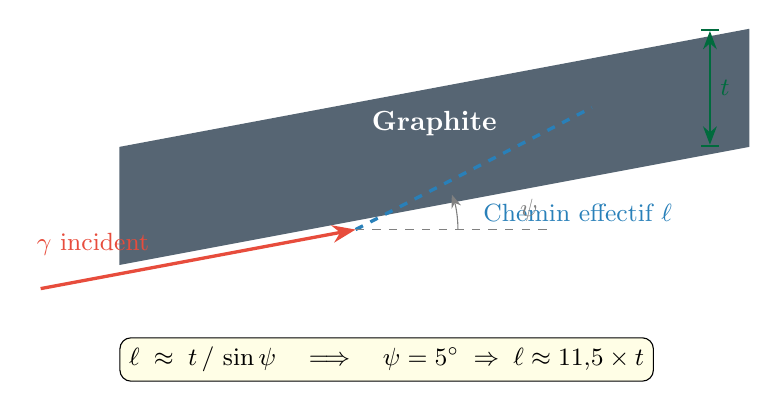
\begin{tikzpicture}[scale=1.0, >=Stealth]
  % Graphite wall (thick slab, tilted)
  \fill[graphite!80] (0,0) -- (8,1.5) -- (8,3.0) -- (0,1.5) -- cycle;
  \node[white, font=\bfseries] at (4,1.8) {Graphite};

  % Incoming ray (grazing)
  \draw[photored, very thick, ->] (-1,-0.3) -- (3,0.45);
  \node[photored, font=\small, above left] at (0.5,0) {$\gamma$ incident};

  % Path through wall
  \draw[comptonblue, very thick, dashed] (3,0.45) -- (6,2.0);
  \node[comptonblue, font=\small, below right] at (4.5,0.9)
    {Chemin effectif $\ell$};

  % Radial thickness
  \draw[|<->|, MyGreen2, thick] (7.5,1.5) -- node[right, font=\small] {$t$} (7.5,3.0);

  % Angles
  \draw[gray, thin, dashed] (3,0.45) -- (5.5,0.45);
  \draw[gray, ->] (4.3,0.45) arc[start angle=0, end angle=20, radius=1.3];
  \node[gray, font=\small] at (5.2,0.7) {$\psi$};

  % Formula
  \node[draw, fill=yellow!10, rounded corners, font=\small, anchor=west] at (0,-1.2)
    {$\ell \;\approx\; t \,/\, \sin\psi \quad\Longrightarrow\quad
      \psi = 5^\circ \;\Rightarrow\; \ell \approx 11{,}5 \times t$};
\end{tikzpicture}
\end{center}

\noindent Pour un photon \'emis \`a $\theta \approx 8^\circ$ (proche du demi-angle du c\^one $\alpha = 7{,}6^\circ$), l'angle d'incidence sur la paroi est $\psi = \theta - \alpha \approx 0{,}4^\circ$, donnant un chemin de plusieurs centim\`etres
dans le graphite~! Cela augmente dramatiquement la probabilit\'e d'interaction Compton.\par

%==============================================================================
\normalsize
\noindent \begin{mdframed}[backgroundcolor=orange!20]
\section{\Large \color{blue} \textbf{Estimation quantitative du gain}\color{black}}
\end{mdframed}
\footnotesize
%==============================================================================

%===============================================================================
\normalsize
\noindent \begin{mdframed}[backgroundcolor=orange!20]
\subsection{\color{blue}\textbf{Bilan des photons}\color{black}}
\end{mdframed}
\footnotesize
%===============================================================================
\medskip

\noindent Pour \num{5000000} photons primaires~:\par

\begin{table}[H]
\centering
\captionsetup{labelformat=empty}
\caption{\footnotesize \textit{Budget de photons estim\'e pour le c\^one graphite}}
\begin{tabular}{@{}l r l@{}}
\toprule
\footnotesize \textbf{Cat\'egorie}&\footnotesize \textbf{Estimation}&\footnotesize \textbf{Note} \\
\midrule
\footnotesize Transmis direct ($\theta < 3{,}2^\circ$)
  &\footnotesize  $\sim$\num{39000}&\footnotesize Identique \`a la r\'ef\'erence \\[4pt]
\footnotesize Interceptent le c\^one ($3{,}2^\circ < \theta < 30^\circ$)
  &\footnotesize  $\sim$\num{130000}&\footnotesize Grande acceptance angulaire \\
\footnotesize \quad$\to$ Compton forward&\footnotesize $\sim$\numrange{2500}{15000}&\footnotesize Redirig\'es vers le plan \\
\footnotesize \quad$\to$ Photo-absorb\'es&\footnotesize  $\sim$\numrange{25000}{75000}&\footnotesize Perdus dans le graphite \\
\footnotesize \quad$\to$ Traversent la paroi&\footnotesize  $\sim$\numrange{50000}{100000}&\footnotesize Absorb\'es par l'inox \\[4pt]
\footnotesize Grand angle ($\theta > 30^\circ$)
  &\footnotesize $\sim$\num{4830000}&\footnotesize Absorb\'es (inox + graphite) \\
\midrule
\footnotesize \textbf{Total sur ScorePlane1}&\footnotesize $\sim$\numrange{42000}{54000}&\footnotesize \textbf{Gain $\times 1{,}1$ \`a $\times 1{,}4$} \\
\bottomrule
\end{tabular}
\end{table}
\noindent \footnotesize \textit{Note~: ces estimations sont analytiques et approximatives. Seule la simulation Monte Carlo donnera la r\'eponse d\'efinitive.}\par

\medskip

\begin{figure}[H]
\centering
\includegraphics[width=1.\textwidth]{Figures/fig_gain_estimation.png}
\captionsetup{labelformat=empty}
\caption{\footnotesize \textit{\textbf{(a)}~Acceptance angulaire~: le c\^one graphite capture les photons jusqu'\`a $\sim$58$^\circ$ (quasi-totalit\'e du c\^one d'\'emission), alors que le cone actuel ne laisse passer que $\theta < 4{,}9^\circ$.
\textbf{(b)}~Budget de flux estim\'e pour 5M primaires. Le gain principal vient des photons Compton forward et de la fuite \`a travers la paroi mince.}}
\end{figure}

%===============================================================================
\normalsize
\noindent \begin{mdframed}[backgroundcolor=orange!20]
\subsection{\color{blue}\textbf{Comparaison synth\'etique}\color{black}}
\end{mdframed}
\footnotesize
%===============================================================================
\medskip

\begin{table}[H]
\centering
\captionsetup{labelformat=empty}
\caption{\footnotesize R\'ef\'erence actuelle vs c\^one graphite (pr\'edictions).}
\renewcommand{\arraystretch}{1.2}
\begin{tabular}{@{}>{\bfseries}p{4cm} c c@{}}
\toprule
 &\footnotesize \textbf{R\'ef\'erence}&\footnotesize \textbf{C\^one graphite} \\
 &\footnotesize (Al + Laiton) &\footnotesize (pr\'edit) \\
\midrule
\footnotesize Collimateur&\footnotesize Cylindre $\varnothing$ 3\,mm&\footnotesize C\^one 6$\to$2\,mm \\
\footnotesize Mat\'eriau&\footnotesize Al ($Z{=}13$) + Laiton ($Z{\approx}29$)&\footnotesize  Graphite ($Z{=}6$) \\
\footnotesize Transmis/5M&\footnotesize  \num{39218}&\footnotesize $\sim$\numrange{42000}{54000} \\
\footnotesize Taux transm&\footnotesize  0,78\%&\footnotesize $\sim$0,8--1,1\% \\
\footnotesize Compton&\footnotesize  \textbf{0}&\footnotesize $\gg 0$ \\
\footnotesize $\Delta E$ Compton &\footnotesize  ---&\footnotesize  $< 2$\% \`a 10\,keV \\
\footnotesize Dose eau &\footnotesize 31,4 nGy&\footnotesize $\uparrow$ attendu \\
\bottomrule
\end{tabular}
\end{table}

%==============================================================================
\normalsize
\noindent \begin{mdframed}[backgroundcolor=orange!20]
\section{\Large \color{blue} \textbf{Impl\'ementation Geant4}\color{black}}
\end{mdframed}
\footnotesize
%==============================================================================

\begin{table}[H]
\centering
\captionsetup{labelformat=empty}
\caption{\footnotesize Modifications apport\'ees au code source Geant4.}
\small
\begin{tabular}{@{}c l p{7.5cm}@{}}
\toprule
\footnotesize \textbf{\#}&\footnotesize \textbf{Fichier}&\footnotesize \textbf{Modification} \\
\midrule
\footnotesize 1&\footnotesize \texttt{.hh}&\footnotesize Ajout du membre \texttt{G4Material* MyGraphite} \\
\footnotesize 2&\footnotesize \texttt{.cc}, \texttt{DefineMaterial()}&\footnotesize Chargement de
    \texttt{"G4\_GRAPHITE"} via le NIST Manager \\
\footnotesize 3&\footnotesize \texttt{.cc}, \texttt{ConstructGDML()}&\footnotesize Remplacement des sections
    Al\,3\,mm et Laiton\,3\,mm par un \texttt{G4Cons} param\'etrique \\
\bottomrule
\end{tabular}
\end{table}

\noindent Le solide \texttt{G4Cons} (c\^one tronqu\'e creux) est d\'efini par~:\par

\begin{verbatim}
  new G4Cons("solidConeCompton",
    coneRinEntry,  coneRout,    // Rmin1, Rmax1 (source)
    coneRinExit,   coneRout,    // Rmin2, Rmax2 (détecteur)
    coneHalfLen, 0.*deg, 360.*deg);
\end{verbatim}

\noindent Pour tester un autre mat\'eriau, il suffit de modifier une seule ligne~:\par

\begin{verbatim}
  G4Material* coneMaterial = MyGraphite;
  // Alternatives :
  // -> nist->FindOrBuildMaterial("G4_PLEXIGLASS");
  // -> nist->FindOrBuildMaterial("G4_POLYETHYLENE");
  // -> nist->FindOrBuildMaterial("G4_BORON_CARBIDE");
\end{verbatim}


%==============================================================================
\normalsize
\noindent \begin{mdframed}[backgroundcolor=orange!20]
\section{\Large \color{blue} \textbf{Diff\'erenciation des primaires directs et des primaires redirig\'es par diffusion Compton}\color{black}}
\end{mdframed}
\footnotesize
%==============================================================================

%============================================================================
\normalsize
\noindent \begin{mdframed}[backgroundcolor=orange!20]
\subsection{\color{blue}\textbf{Contexte et motivation}\color{black}}
\end{mdframed}
\footnotesize
%===============================================================================
\medskip

\noindent Dans Geant4, lorsqu'un photon $\gamma$ primaire subit une diffusion Compton, le \color{blue}\textbf{photon diffus\'e continue comme le m\^eme track}\color{black} \; (m\^eme \color{blue}\textbf{trackID}\color{black}, \color{blue}\textbf{parentID~=~0}\color{black}).\par
\noindent \normalsize$\bm{\longrightarrow}$\footnotesize Seul l'\'electron de recul est cr\'e\'e en tant que secondaire (\color{blue}\textbf{creator\_process~=~"compt"}\color{black}).
\medskip
\begin{tcolorbox}[colback=white, colframe=blue, title=Cons\'equence, fonttitle=\bfseries]
\noindent Au ScorePlane ($\bm{z} = \bm{18}$~mm), un photon redirig\'e par Compton dans le c\^one graphite est \color{blue}\textbf{indiscernable}\color{black} \; d'un photon transmis directement \`a travers le canal.\par
\noindent Les deux apparaissent comme \color{blue}\textbf{parentID~=~0}\color{black}, \color{blue}\textbf{creator\_process~=~"primary"}\color{black}.
\end{tcolorbox}
\medskip
\begin{tcolorbox}[colback=white, colframe=blue, title=Objectif, fonttitle=\bfseries]
\noindent Ajouter un marquage (flag) sur le track primaire pour distinguer les trois populations au ScorePlane\par
\end{tcolorbox}


\begin{center}
\renewcommand{\arraystretch}{1.2}
\begin{tabular}{clcc}
\toprule
\footnotesize \textbf{Cat.}&\footnotesize \textbf{Description}&\footnotesize \texttt{parentID}&\footnotesize \texttt{compton\_in\_cone} \\
\midrule
\footnotesize A&\footnotesize Primaire transmis directement&\footnotesize 0&\footnotesize 0\\
\footnotesize B&\footnotesize Primaire redirig\'e par Compton&\footnotesize 0&\footnotesize  1\\
\footnotesize C&\footnotesize Secondaire (e$^-$, $\gamma$ Brem\dots)&\footnotesize $\geq 1$&\footnotesize  ---\\
\bottomrule
\end{tabular}
\end{center}

%============================================================================
\normalsize
\noindent \begin{mdframed}[backgroundcolor=orange!20]
\subsection{\color{blue}\textbf{Fichiers modifi\'es}\color{black}}
\end{mdframed}
\footnotesize
%===============================================================================
\medskip

\begin{center}
\renewcommand{\arraystretch}{1.2}
\begin{tabular}{lll}
\toprule
\footnotesize \textbf{Fichier}&\footnotesize \textbf{R\'epertoire}&\footnotesize \textbf{Nature de la modification} \\
\midrule 
\footnotesize \texttt{MyTrackInfo.hh}&\footnotesize \texttt{include/}&\footnotesize Ajout champs Compton \\
\footnotesize \texttt{MyTrackInfo.cc}&\footnotesize \texttt{src/}&\footnotesize Initialisation des nouveaux champs \\
\footnotesize \texttt{SteppingAction.cc}&\footnotesize \texttt{src/}&\footnotesize D\'etection Compton dans le c\^one \\
\footnotesize \texttt{AnalysisManagerSetup.cc}&\footnotesize \texttt{src/}&\footnotesize 5 nouvelles colonnes ntuple \\
\footnotesize \texttt{SurfaceSpectrumSD.cc}&\footnotesize \texttt{src/}&\footnotesize Lecture flag + remplissage ntuple \\
\bottomrule
\end{tabular}
\end{center}

\noindent Aucun autre fichier n'est modifi\'e. Les fichiers \texttt{.hh} et \texttt{.cc} non list\'es ci-dessus restent inchang\'es.\par

%===============================================================================
\normalsize
\noindent \begin{mdframed}[backgroundcolor=orange!20]
\subsection{\color{blue}\textbf{D\'etail des modifications}\color{black}}
\end{mdframed}
\footnotesize
%===============================================================================
\medskip

%===============================================================================
\normalsize
\noindent \color{blue}\textbf{MyTrackInfo.hh / .cc $\bm{\longrightarrow}$ Stockage de l'information Compton}\color{black}
\footnotesize
%===============================================================================
\smallskip
\noindent \color{blue}\textbf{Quatre nouveaux champs priv\'es}\color{black} \; sont ajout\'es \`a la classe \color{blue}\textbf{MyTrackInfo}\color{black} \; (qui h\'erite de \color{blue}\textbf{G4VUserTrackInformation}\color{black} \; et est attach\'ee \`a chaque \color{blue}\textbf{track}\color{black}) :\par

\begin{center}
\renewcommand{\arraystretch}{1.15}
{\small
\begin{tabular}{llll}
\toprule
\footnotesize \textbf{Champ}&\footnotesize \textbf{Type}&\footnotesize \textbf{Init.}&\footnotesize \textbf{Description}\\
\midrule
\footnotesize\texttt{fComptonInCone}&\footnotesize \texttt{G4bool}&\footnotesize \texttt{false}&\footnotesize Flag : $\geq 1$ Compton dans le c\^one \\
\footnotesize\texttt{fNComptonInCone}&\footnotesize \texttt{G4int}&\footnotesize \texttt{0}&\footnotesize Nombre total de Compton dans le c\^one \\
\footnotesize\texttt{fLastComptonPos}&\footnotesize \texttt{G4ThreeVector}&\footnotesize \texttt{(0,0,0)}&\footnotesize Position de la derni\`ere diffusion \\
\footnotesize\texttt{fLastComptonEkin}&\footnotesize \texttt{G4double}&\footnotesize \texttt{0.}&\footnotesize $E_{\mathrm{kin}}$ avant la derni\`ere diffusion \\
\bottomrule
\end{tabular}
}
\end{center}
\noindent $\bullet$ Accesseurs publics correspondants : \texttt{Set/Get/Has} + \texttt{IncrementNComptonInCone()}.\par
\noindent $\bullet$ L'include \texttt{G4ThreeVector.hh} est ajout\'e en en-t\^ete.\par

\medskip
%===============================================================================
\normalsize
\noindent \color{blue}\textbf{SteppingAction.cc $\bm{\longrightarrow}$ D\'etection du Compton dans le c\^one}\color{black}
\footnotesize
%===============================================================================
\smallskip
\noindent Un nouveau bloc est ins\'er\'e dans \color{blue}\textbf{UserSteppingAction()}\color{black}, juste apr\`es la r\'ecup\'eration des noms de mat\'eriaux (\texttt{matNamePre}, \texttt{matNamePost}).\par
\medskip
\noindent \color{blue}\textbf{Condition de d\'eclenchement}\color{black} \; (les 3 conditions doivent \^etre vraies simultan\'ement) :\par
\begin{enumerate}[nosep]
\item Le processus d\'efini au post-step est \texttt{"compt"}
\item Le volume logique au pr\'e-step est \texttt{"logicConeCompton"}
\item Le track est un primaire (\texttt{parentID == 0})
\end{enumerate}
\smallskip
\noindent \color{blue}\textbf{Actions :}\color{black}\par
\begin{enumerate}[nosep]
\item \texttt{info->SetComptonInCone(true)}
\item \texttt{info->IncrementNComptonInCone()}
\item \texttt{info->SetLastComptonPos(postPoint->GetPosition())}
\item \texttt{info->SetLastComptonEkin(prePoint->GetKineticEnergy())}
\end{enumerate}
\smallskip
\noindent \color{blue}\textbf{Log :}\color{black}\par
\begin{enumerate}[nosep]
\item tag \texttt{[STEP][COMPTON\_IN\_CONE]}
\item 100 premiers puis 1 sur 10\,000.
\item Prot\'eg\'e par mutex (\texttt{G4AutoLock}) pour la compatibilit\'e multi-thread.
\end{enumerate}
\smallskip
\begin{lstlisting}[style=cpp, title={\footnotesize \textit{Extrait de \textbf{SteppingAction.cc} (bloc ajout\'e)}}]
const G4VProcess* procDefined = postPoint->GetProcessDefinedStep();
if (procDefined && track->GetParentID() == 0
    && procDefined->GetProcessName() == "compt"
    && namePre == "logicConeCompton")
{
    MyTrackInfo* info =
        static_cast<MyTrackInfo*>(track->GetUserInformation());
    if (info) {
        info->SetComptonInCone(true);
        info->IncrementNComptonInCone();
        info->SetLastComptonPos(postPoint->GetPosition());
        info->SetLastComptonEkin(prePoint->GetKineticEnergy());
    }
}
\end{lstlisting}

\medskip
%===============================================================================
\normalsize
\noindent \color{blue}\textbf{AnalysisManagerSetup.cc $\bm{\longrightarrow}$ Nouvelles colonnes du ntuple}\color{black}
\footnotesize
%===============================================================================
\smallskip

\noindent Cinq colonnes sont ajout\'ees au ntuple \color{blue}\textbf{plane\_passages}\color{black} (indices 10 \`a 14), juste avant le \color{blue}\textbf{FinishNtuple}\color{black} :

\begin{lstlisting}[style=cpp, title={\footnotesize \textit{Colonnes ajout\'ees dans \textbf{AnalysisManagerSetup.cc}}}]
// [ADD] Colonnes Compton dans le cone graphite
CreateNtupleIColumn(id, "compton_in_cone"); // 10
CreateNtupleIColumn(id, "n_compton_cone");  // 11
CreateNtupleDColumn(id, "compton_x_mm");    // 12
CreateNtupleDColumn(id, "compton_y_mm");    // 13
CreateNtupleDColumn(id, "compton_z_mm");    // 14
\end{lstlisting}

\medskip
%===============================================================================
\normalsize
\noindent \color{blue}\textbf{SurfaceSpectrumSD.cc $\bm{\longrightarrow}$  Lecture du flag et remplissage}\color{black}
\footnotesize
%===============================================================================
\smallskip
\noindent Dans \color{blue}\textbf{ProcessHits()}\color{black}, apr\`es le calcul de \color{blue}\textbf{is\_secondary}\color{black} :\par
\begin{enumerate}[nosep]
\item R\'ecup\'eration du \texttt{MyTrackInfo} attach\'e au track
\item Lecture de \texttt{HasComptonInCone()}, \texttt{GetNComptonInCone()}, \texttt{GetLastComptonPos()}
\item Remplissage des colonnes 10--14 du ntuple
\item Log \texttt{[ScorePlane1][COMPTON\_REDIRECTED]} (200 premiers puis 1 sur 5\,000)
\end{enumerate}

\noindent L'include \color{blue}\textbf{MyTrackInfo.hh}\color{black} \; est ajout\'e en en-t\^ete du fichier.\par

%==============================================================================
\normalsize
\noindent \begin{mdframed}[backgroundcolor=orange!20]
\section{\Large \color{blue} \textbf{Structure compl\`ete du ntuple \texttt{plane\_passages}}\color{black}}
\end{mdframed}
\footnotesize
%==============================================================================
% ===================================================================
%  STRUCTURE COMPLETE DU NTUPLE
% ===================================================================

\begin{table}[H]
\centering
\captionsetup{labelformat=empty}
\caption{\footnotesize Colonnes du ntuple \color{blue}\textbf{plane\_passages}\color{black} (ScorePlane, $\bm{z} = 18$~mm).
Les colonnes 0--9 sont inchang\'ees.
Les colonnes 10--14 (sur fond vert) sont ajout\'ees.}
\renewcommand{\arraystretch}{1.2}
{\small
\begin{tabular}{ccllp{6.5cm}}
\toprule
\footnotesize \textbf{Col.} &\footnotesize  \textbf{Type} &\footnotesize  \textbf{Nom} &\footnotesize  \textbf{Unit\'e} &\footnotesize  \textbf{Description} \\
\midrule
\footnotesize 0&\footnotesize \texttt{int}   &\footnotesize \texttt{pdg}             &\footnotesize ---& Code PDG (22 = $\gamma$, 11 = $e^-$) \\
\footnotesize 1&\footnotesize \texttt{string}&\footnotesize \texttt{name}            &\footnotesize ---& Nom de la particule \\
\footnotesize 2&\footnotesize \texttt{int}   &\footnotesize \texttt{is\_secondary}   &\footnotesize ---& 0 = primaire, 1 = secondaire \\
\footnotesize 3&\footnotesize \texttt{double}&\footnotesize \texttt{x\_mm}           &\footnotesize mm & Position $x$ au plan \\
\footnotesize 4&\footnotesize \texttt{double}&\footnotesize \texttt{y\_mm}           &\footnotesize mm & Position $y$ au plan \\
\footnotesize 5&\footnotesize \texttt{double}&\footnotesize \texttt{z\_mm}           &\footnotesize mm & Position $z$ au plan ($\approx 18$) \\
\footnotesize 6&\footnotesize \texttt{double}&\footnotesize \texttt{ekin\_keV}       &\footnotesize keV& \'Energie cin\'etique au plan \\
\footnotesize 7&\footnotesize \texttt{int}   &\footnotesize \texttt{trackID}         &\footnotesize ---& Identifiant du track \\
\footnotesize 8&\footnotesize \texttt{int}   &\footnotesize \texttt{parentID}        &\footnotesize ---& ID du parent (0 = primaire) \\
\footnotesize 9&\footnotesize \texttt{string}&\footnotesize \texttt{creator\_process}&\footnotesize --- & Processus cr\'eateur \\
\midrule
\rowcolor{addgreen}
\footnotesize 10&\footnotesize \texttt{int}&\footnotesize \texttt{compton\_in\_cone}&\footnotesize ---&\footnotesize 1 si $\geq 1$ Compton dans le c\^one, 0 sinon \\
\rowcolor{addgreen}
\footnotesize 11&\footnotesize \texttt{int}&\footnotesize \texttt{n\_compton\_cone}&\footnotesize ---&\footnotesize Nombre de diffusions Compton dans le c\^one \\
\rowcolor{addgreen}
\footnotesize 12&\footnotesize \texttt{double}&\footnotesize \texttt{compton\_x\_mm}&\footnotesize mm&\footnotesize $x$ de la derni\`ere diffusion Compton \\
\rowcolor{addgreen}
\footnotesize 13&\footnotesize \texttt{double}&\footnotesize \texttt{compton\_y\_mm}&\footnotesize mm&\footnotesize $y$ de la derni\`ere diffusion Compton \\
\rowcolor{addgreen}
\footnotesize 14&\footnotesize \texttt{double}&\footnotesize \texttt{compton\_z\_mm}&\footnotesize mm&\footnotesize $z$ de la derni\`ere diffusion Compton \\
\bottomrule
\end{tabular}
}
\end{table}
\begin{itemize}[nosep]
\item Les colonnes 12--14 valent $(0, 0, 0)$ si \texttt{compton\_in\_cone~=~0}.
\item Si le photon subit plusieurs Compton dans le c\^one (\texttt{n\_compton\_cone~$> 1$}), seule la position de la \emph{derni\`ere} diffusion est enregistr\'ee.
\item Les ntuples des autres plans (ScorePlane2, 3, 5) ne sont \color{blue}\textbf{pas modifi\'es}\color{black}.
\end{itemize}


%==============================================================================
\normalsize
\noindent \begin{mdframed}[backgroundcolor=orange!20]
\section{\Large \color{blue} \textbf{Classification des particules au ScorePlane}\color{black}}
\end{mdframed}
\footnotesize
%==============================================================================

% ===================================================================
%  CLASSIFICATION DES PARTICULES
% ===================================================================


\begin{table}[H]
\centering
\captionsetup{labelformat=empty}
\caption{\footnotesize Classification des particules au ScorePlane.}
\renewcommand{\arraystretch}{1.3}
{\small
\begin{tabular}{p{3.8cm}cccp{4.5cm}}
\toprule
\scriptsize \textbf{Cat\'egorie}&\scriptsize \texttt{parentID}&\scriptsize \texttt{is\_sec}&\scriptsize \texttt{compton\_in\_cone}&\scriptsize \textbf{Filtre ROOT} \\
\midrule
\scriptsize Primaire transmis directement ($\theta < 3.4°$)&\scriptsize 0 &\scriptsize 0 &\scriptsize 0&\scriptsize \texttt{is\_secondary==0 \&\& compton\_in\_cone==0} \\
\scriptsize Primaire redirig\'e Compton&\scriptsize 0 &\scriptsize 0 &\scriptsize 1&\scriptsize \texttt{is\_secondary==0 \&\& compton\_in\_cone==1} \\
\scriptsize Secondaire (photo\'electron, Brem\dots)&\scriptsize $\geq 1$ &\scriptsize 1 &\scriptsize --- &\scriptsize \texttt{is\_secondary==1} \\
\bottomrule
\end{tabular}
}
\end{table}
\noindent Avec les nouvelles colonnes, chaque entr\'ee du ntuple peut \^etre class\'ee sans ambigu\"it\'e :

%==============================================================================
\normalsize
\noindent \begin{mdframed}[backgroundcolor=orange!20]
\section{\Large \color{blue} \textbf{Nouveaux tags dans le fichier \texttt{.log}}\color{black}}
\end{mdframed}
\footnotesize
%==============================================================================

% ===================================================================
% TAGS DE LOG
% ===================================================================

\begin{table}[H]
\centering
\captionsetup{labelformat=empty}
\caption{\footnotesize \textit{Tags de log ajout\'es.}}
\renewcommand{\arraystretch}{1.2}
{\small
\begin{tabular}{lllp{2.5cm}}
\toprule
\footnotesize \textbf{Tag} &\footnotesize \textbf{Source} & \footnotesize\textbf{Fr\'equence} &\footnotesize \textbf{Contenu} \\
\midrule
\scriptsize\texttt{[STEP][COMPTON\_IN\_CONE]}
  &\scriptsize \texttt{SteppingAction}
  &\scriptsize 100 premiers, puis 1/10\,000
  &\scriptsize \'Ev\'enement, trackID, $n_{\mathrm{compt}}$,$E_{\mathrm{avant}}$,$E_{\mathrm{apr\grave{e}s}}$, position \\[4pt]
\scriptsize\texttt{[ScorePlane1][COMPTON\_REDIRECTED]}
  &\scriptsize \texttt{SurfaceSpectrumSD}
  &\scriptsize 200 premiers, puis 1/5\,000
  &\scriptsize Particule, trackID, $E$ au plan, $n_{\mathrm{compt}}$, position Compton, position au plan \\
\bottomrule
\end{tabular}
}
\end{table}

%==============================================================================
\normalsize
\noindent \begin{mdframed}[backgroundcolor=orange!20]
\section{\Large \color{blue} \textbf{Exemples d'analyse ROOT}\color{black}}
\end{mdframed}
\footnotesize
%==============================================================================

% ===================================================================
% EXEMPLES D'ANALYSE ROOT
% ===================================================================

\begin{lstlisting}[style=root, title={\footnotesize \textit{Exemples de commandes ROOT/TTree::Draw}}]
// Spectre en energie des photons transmis directement
plane_passages->Draw("ekin_keV",
    "pdg==22 && is_secondary==0 && compton_in_cone==0")

// Spectre en energie des photons rediriges par Compton
plane_passages->Draw("ekin_keV",
    "pdg==22 && is_secondary==0 && compton_in_cone==1")

// Distribution en z des lieux de diffusion Compton
plane_passages->Draw("compton_z_mm",
    "compton_in_cone==1")

// Distribution radiale r = sqrt(x^2+y^2) des Compton
plane_passages->Draw("sqrt(compton_x_mm^2+compton_y_mm^2)",
    "compton_in_cone==1")

// Perte d'energie fractionnelle par Compton (si >0)
plane_passages->Draw("n_compton_cone",
    "compton_in_cone==1")

// Comptages
plane_passages->Draw("compton_in_cone",
    "pdg==22 && is_secondary==0")
// -> bin 0 = transmis directs, bin 1 = Compton rediriges
\end{lstlisting}

\clearpage

%==============================================================================
\normalsize
\noindent \begin{mdframed}[backgroundcolor=orange!20]
\section{\Large \color{blue} \textbf{Sch\'ema synoptique du flux de donn\'ees}\color{black}}
\end{mdframed}
\footnotesize
%==============================================================================

% ===================================================================
%  SCHEMA SYNOPTIQUE
% ===================================================================

\begin{center}
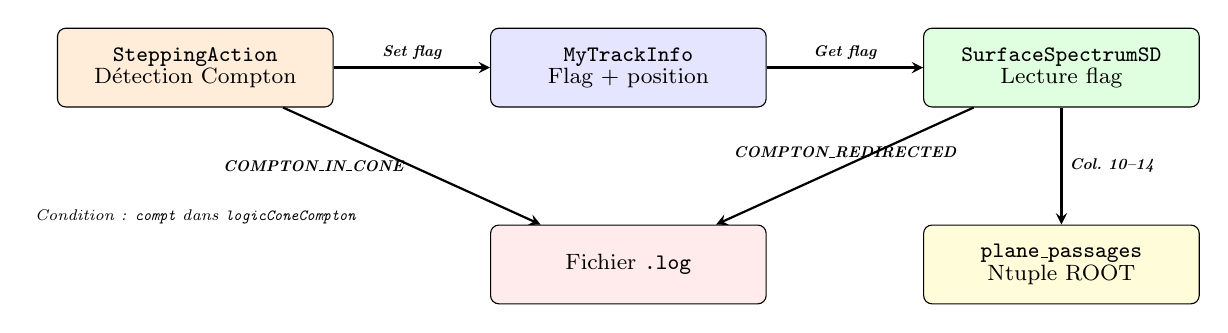
\begin{tikzpicture}[
  box/.style={draw, rounded corners=3pt, minimum height=1cm, minimum width=3.5cm,
              align=center, font=\scriptsize},
  arrow/.style={->, >=stealth, thick},
  note/.style={font=\scriptsize\itshape, scale=0.8,text=black},
]
% Boîtes
\node[box, fill=orange!15] (step) at (0,0) {\footnotesize \texttt{SteppingAction}\\\footnotesize D\'etection Compton};
\node[box, fill=blue!10]   (info) at (5.5,0) {\texttt{\footnotesize MyTrackInfo}\\\footnotesize Flag + position};
\node[box, fill=green!12]  (sd)   at (11,0) {\footnotesize \texttt{SurfaceSpectrumSD}\\\footnotesize Lecture flag};
\node[box, fill=yellow!15] (nt)   at (11,-2.5) {\footnotesize \texttt{plane\_passages}\\\footnotesize Ntuple ROOT};
\node[box, fill=red!8]     (log)  at (5.5,-2.5) {\footnotesize Fichier \texttt{.log}};

% Flèches
\draw[arrow] (step) -- node[above, note] {\textbf{Set flag}} (info);
\draw[arrow] (info) -- node[above, note] {\textbf{Get flag}} (sd);
\draw[arrow] (sd)   -- node[right, note] {\textbf{Col.\ 10--14}} (nt);
\draw[arrow] (step) -- node[left, note] {\scriptsize \textbf{COMPTON\_IN\_CONE}} (log);
\draw[arrow] (sd)   -- node[above, note] {\scriptsize \textbf{COMPTON\_REDIRECTED}} (log);

% Annotation processus
\node[note, anchor=north] at (0, -1.7) {Condition : \texttt{compt} dans \texttt{logicConeCompton}};
\end{tikzpicture}
\end{center}

%==============================================================================
\normalsize
\noindent \begin{mdframed}[backgroundcolor=orange!20]
\section{\Large \color{blue} \textbf{Enregistrement des photoabsorptions de primaires dans le graphite et l'inox}\color{black}}
\end{mdframed}
\footnotesize
%==============================================================================

%===============================================================================
\normalsize
\noindent \begin{mdframed}[backgroundcolor=orange!20]
\subsection{\color{blue}\textbf{Contexte et objectif}\color{black}}
\end{mdframed}
\footnotesize
%===============================================================================
\medskip

\noindent Le code existant comptabilisait les pertes de primaires par processus et par mat\'eriau dans des maps globales (\texttt{gLostByProc}, \texttt{gLostByMat}), imprim\'ees en fin de run sous les tags \texttt{[LOSS][BY-PROC]} et \texttt{[LOSS][BY-MAT]}.\par

\noindent Ce m\'ecanisme fournissait des \color{blue}\textbf{totaux agr\'eg\'es}\color{black} \; mais aucune information \'ev\'enement par \'ev\'enement (position, \'energie, volume logique exact).\par 

\medskip

\begin{tcolorbox}[colback=white, colframe=blue, title=Objectif, fonttitle=\bfseries]
\noindent Cr\'eer \color{blue}\textbf{deux ntuples}\color{black} \; ROOT d\'edi\'es enregistrant \color{blue}\textbf{chaque absorption photo\'electrique}\color{black} \;  individuelle d'un $\gamma$ primaire :\par
\begin{itemize}[nosep]
\item \color{blue}\textbf{abs\_graphite}\color{black} $\longrightarrow$ absorptions dans le c\^one graphite (\texttt{logicConeCompton})
\item \color{blue}\textbf{abs\_inox}\color{black} $\longrightarrow$ absorptions dans l'inox SS304 (porte-collimateur et enveloppe tube)
\end{itemize}
\noindent Chaque entr\'ee conserve \color{blue}\textbf{la position}\color{black} \; $(\bm{x},\bm{y},\bm{z})$, \color{blue}\textbf{l'\'energie cin\'etique}\color{black} \; au moment de l'absorption, et \color{blue}\textbf{l'historique Compton}\color{black} \; dans le c\^one (flag + compteur), permettant de corr\'eler absorption et diffusion ant\'erieure.\par
\end{tcolorbox}

%===============================================================================
\normalsize
\noindent \begin{mdframed}[backgroundcolor=orange!20]
\subsection{\color{blue}\textbf{Fichiers modifi\'es}\color{black}}
\end{mdframed}
\footnotesize
%===============================================================================
\medskip
% ===================================================================
%  FICHIERS MODIFIES
% ===================================================================

\noindent \color{blue}\textbf{Trois fichiers}\color{black} \; sont concern\'es par cet ajout. Les modifications pr\'ec\'edentes (tracking Compton via \texttt{MyTrackInfo}, sont un pr\'erequis.\par

\begin{table}[H]
\centering
\renewcommand{\arraystretch}{1.2}
\begin{tabular}{lll}
\toprule
\footnotesize \textbf{Fichier}&\footnotesize \textbf{R\'ep.}&\footnotesize \textbf{Nature de la modification}\\
\midrule
\footnotesize \texttt{AnalysisManagerSetup.hh}&\footnotesize \texttt{include/}&\footnotesize D\'eclarations des getters des 2 nouveaux ntuples \\
\footnotesize \texttt{AnalysisManagerSetup.cc}&\footnotesize \texttt{src/}&\footnotesize Cr\'eation des 2 ntuples + getters\\
\footnotesize \texttt{SteppingAction.cc}&\footnotesize \texttt{src/}&\footnotesize Remplissage des ntuples \`a la mort du primaire\\
\bottomrule
\end{tabular}
\end{table}

\noindent Les fichiers \texttt{MyTrackInfo.hh/.cc} et \texttt{SurfaceSpectrumSD.cc} ne requi\`erent \color{blue}\textbf{aucune modification suppl\'ementaire}\color{black} \; par rapport \`a la synth\`ese pr\'ec\'edente.\par

%===============================================================================
\normalsize
\noindent \begin{mdframed}[backgroundcolor=orange!20]
\subsection{\color{blue}\textbf{D\'etail des modifications}\color{black}}
\end{mdframed}
\footnotesize
%===============================================================================
% ===================================================================
%  DETAIL DES MODIFICATIONS
% ===================================================================
\medskip
%===============================================================================
\normalsize
\noindent \color{blue}\textbf{\texttt{AnalysisManagerSetup.hh / .cc} --- Cr\'eation des ntuples}\color{black}
\footnotesize
%===============================================================================
\smallskip
\noindent \textbf{En-t\^ete (\texttt{.hh})}\par
\noindent Deux nouvelles d\'eclarations de fonctions getter :\par
\begin{lstlisting}[style=cpp, title={\footnotesize \textit{Ajouts dans \texttt{AnalysisManagerSetup.hh}}}]
int GetAbsGraphiteNtupleId();
int GetAbsInoxNtupleId();
\end{lstlisting}

\noindent \textbf{Source (\texttt{.cc})}\par
\noindent Deux variables statiques, deux blocs \texttt{CreateNtuple} et deux getters sont ajout\'es.\par
\noindent Le ntuple \texttt{abs\_graphite} comporte 8 colonnes (indices 0--7) et le ntuple \texttt{abs\_inox} en comporte 9 (indices 0--8), la colonne suppl\'ementaire \'etant le nom du volume logique (pour distinguer porte-collimateur d'enveloppe).\par

\medskip
%===============================================================================
\normalsize
\noindent \color{blue}\textbf{\texttt{SteppingAction.cc} --- D\'etection et remplissage}\color{black}
\footnotesize
%===============================================================================
\smallskip
\noindent \textbf{Nouvel include}\par
\begin{lstlisting}[style=cpp, title={\footnotesize \textit{Include ajout\'e}}]
#include "AnalysisManagerSetup.hh"
\end{lstlisting}

\noindent \textbf{Logique de remplissage}\par
\noindent Un nouveau bloc \texttt{do \{...\} while(0)} est ins\'er\'e dans la section \texttt{[TRACE] Fin de piste PRIMAIRE}, juste apr\`es le bloc \texttt{[LOSS]} existant (lignes $\sim$1104).\par
\noindent Il se d\'eclenche \textbf{uniquement} quand les conditions suivantes sont \emph{toutes} r\'eunies :\par

\begin{enumerate}[nosep]
\item Le track est un primaire (\texttt{parentID == 0}) --- d\'ej\`a garanti par le bloc parent
\item Le track est mort (\texttt{fStopAndKill}) ou sort du monde
\item Le processus qui a tu\'e le track est \texttt{"phot"} (effet photo\'electrique)
\end{enumerate}

\noindent Ensuite, le volume logique au pr\'e-step d\'etermine dans quel ntuple \'ecrire :\par
\begin{itemize}[nosep]
\item \texttt{namePre == "logicConeCompton"} $\to$ ntuple \texttt{abs\_graphite}
\item \texttt{materialPre == "StainlessSteel304"} $\to$ ntuple \texttt{abs\_inox}
\end{itemize}

\medskip

\begin{lstlisting}[style=cpp, title={\footnotesize \textit{Extrait du bloc de remplissage (cas graphite)}}]
if (!proc || proc->GetProcessName() != "phot") break;

const G4ThreeVector absPos = postPoint->GetPosition();
const G4double abs_ekin_keV = prePoint->GetKineticEnergy()/keV;

// Info Compton depuis MyTrackInfo
G4int had_compton = 0, n_compton = 0;
if (trackInfo) {
    had_compton = trackInfo->HasComptonInCone() ? 1 : 0;
    n_compton   = trackInfo->GetNComptonInCone();
}

if (namePre == "logicConeCompton") {
    const G4int id = GetAbsGraphiteNtupleId();
    man->FillNtupleIColumn(id, 0, eventID);
    man->FillNtupleIColumn(id, 1, track->GetTrackID());
    man->FillNtupleDColumn(id, 2, abs_ekin_keV);
    man->FillNtupleDColumn(id, 3, absPos.x()/mm);
    man->FillNtupleDColumn(id, 4, absPos.y()/mm);
    man->FillNtupleDColumn(id, 5, absPos.z()/mm);
    man->FillNtupleIColumn(id, 6, had_compton);
    man->FillNtupleIColumn(id, 7, n_compton);
    man->AddNtupleRow(id);
}
\end{lstlisting}

\noindent Le cas \color{blue}\textbf{abs\_inox}\color{black} \; est identique, avec en plus la colonne 6 de type \color{blue}\textbf{string}\color{black} \; contenant le nom du volume logique (\texttt{namePre}), ce qui permet de distinguer le porte-collimateur de l'enveloppe inox.\par

\clearpage

%===============================================================================
\normalsize
\noindent \begin{mdframed}[backgroundcolor=orange!20]
\subsection{\color{blue}\textbf{Structure compl\`ete des ntuples}\color{black}}
\end{mdframed}
\footnotesize
%===============================================================================
\medskip
% ===================================================================
%  STRUCTURE DES NTUPLES
% ===================================================================

\medskip
%===============================================================================
\normalsize
\noindent \color{blue}\textbf{Ntuple \texttt{abs\_graphite}}\color{black}
\footnotesize
%===============================================================================
\smallskip

\begin{table}[H]
\centering
\captionsetup{labelformat=empty}
\caption{\footnotesize \textit{Ntuple \texttt{abs\_graphite} --- Photoabsorptions de primaires dans le c\^one graphite (\texttt{logicConeCompton}).}}
\renewcommand{\arraystretch}{1.2}
{\small
\begin{tabular}{ccllp{6.2cm}}
\toprule
\footnotesize \textbf{Col}&\footnotesize \textbf{Type}&\footnotesize \textbf{Nom}&\footnotesize \textbf{Unit\'e}&\footnotesize\textbf{Description} \\
\midrule
\rowcolor{white}
\footnotesize 0&\footnotesize \texttt{int}&\footnotesize \texttt{eventID}&\footnotesize ---&\footnotesize Num\'ero de l'\'ev\'enemen \\
\rowcolor{white}
\footnotesize 1&\footnotesize \texttt{int}&\footnotesize \texttt{trackID}&\footnotesize ---&\footnotesize Identifiant du track \\
\rowcolor{white}
\footnotesize 2&\footnotesize \texttt{double}&\footnotesize \texttt{ekin\_keV}&\footnotesize keV&\footnotesize \'Energie cin\'etique juste avant l'absorption \\
\rowcolor{white}
\footnotesize 3&\footnotesize \texttt{double}&\footnotesize \texttt{x\_mm}&\footnotesize mm&\footnotesize Position $\bm{x}$ de l'absorption \\
\rowcolor{white}
\footnotesize 4&\footnotesize \texttt{double}&\footnotesize \texttt{y\_mm}&\footnotesize mm&\footnotesize Position $\bm{y}$ de l'absorption \\
\rowcolor{white}
\footnotesize 5& \texttt{double}&\footnotesize \texttt{z\_mm}&\footnotesize mm&\footnotesize Position $\bm{z}$ de l'absorption \\
\rowcolor{white}
\footnotesize 6& \texttt{int}&\footnotesize \texttt{had\_compton\_in\_cone}&\footnotesize ---  &\footnotesize 1 si le $\bm{\gamma}$ avait subi $\geq 1$ Compton dans le c\^one \\
\rowcolor{white}
\footnotesize 7& \texttt{int}&\footnotesize \texttt{n\_compton\_in\_cone}&\footnotesize ---&\footnotesize Nombre de Compton dans le c\^one avant absorption \\
\bottomrule
\end{tabular}
}
\end{table}

\medskip

\noindent \textbf{Volume concern\'e :} \texttt{logicConeCompton} uniquement (G4Cons, graphite $\bm{\rho} = 1.7$~g/cm$^3$, $z \in [1.90 ; 16.95]$~mm).\par


\medskip
%===============================================================================
\normalsize
\noindent \color{blue}\textbf{Ntuple \texttt{abs\_inox}}\color{black}
\footnotesize
%===============================================================================
\smallskip

\begin{table}[H]
\centering
\captionsetup{labelformat=empty}
\caption{\footnotesize \textit{Ntuple \texttt{abs\_inox} --- Photoabsorptions de primaires
dans l'inox SS304.}}
\renewcommand{\arraystretch}{1.2}
{\small
\begin{tabular}{ccllp{6.2cm}}
\toprule
\footnotesize\textbf{Col.} &\footnotesize \textbf{Type}&\footnotesize \textbf{Nom}&\footnotesize \textbf{Unit\'e}&\footnotesize \textbf{Description} \\
\midrule
\rowcolor{inox}
\footnotesize 0&\footnotesize \texttt{int}&\footnotesize \texttt{eventID}&\footnotesize ---&\footnotesize Num\'ero de l'\'ev\'enement \\
\rowcolor{inox}
\footnotesize 1&\footnotesize \texttt{int}&\footnotesize \texttt{trackID}&\footnotesize ---&\footnotesize Identifiant du track \\
\rowcolor{inox}
\footnotesize 2&\footnotesize \texttt{double}&\footnotesize \texttt{ekin\_keV}&\footnotesize keV&\footnotesize \'Energie cin\'etique juste avant l'absorption \\
\rowcolor{inox}
\footnotesize 3&\footnotesize \texttt{double}&\footnotesize \texttt{x\_mm}&\footnotesize mm&\footnotesize Position $x$ de l'absorption \\
\rowcolor{inox}
\footnotesize 4&\footnotesize \texttt{double}&\footnotesize \texttt{y\_mm}&\footnotesize mm&\footnotesize\footnotesize Position $y$ de l'absorption \\
\rowcolor{inox}
\footnotesize 5&\footnotesize \texttt{double}&\footnotesize \texttt{z\_mm}&\footnotesize mm&\footnotesize Position $z$ de l'absorption \\
\rowcolor{inox}
\footnotesize 6&\footnotesize \texttt{string} &\footnotesize \texttt{volume}&\footnotesize ---&\footnotesize Nom du volume logique (voir tableau~\ref{tab:volumes_inox}) \\
\rowcolor{inox}
\footnotesize 7&\footnotesize \texttt{int}&\footnotesize \texttt{had\_compton\_in\_cone}&\footnotesize ---&\footnotesize 1 si le $\gamma$ avait subi $\geq 1$ Compton dans le c\^one \\
\rowcolor{inox}
\footnotesize 8&\footnotesize \texttt{int}&\footnotesize \texttt{n\_compton\_in\_cone}&\footnotesize ---&\footnotesize Nombre de Compton dans le c\^one avant absorption \\
\bottomrule
\end{tabular}
}
\end{table}


\begin{table}[H]
\centering
\captionsetup{labelformat=empty}
\caption{\footnotesize \textit{Volumes logiques en inox SS304 distingu\'es par la colonne \texttt{volume}}.}
\renewcommand{\arraystretch}{1.15}
{\small
\begin{tabular}{lll}
\toprule
\footnotesize\textbf{Valeur de \texttt{volume}}&\footnotesize \textbf{Pi\`ece} &\footnotesize \textbf{Description} \\
\midrule
\footnotesize\texttt{logicPorteCollimateur}&\footnotesize Porte-collimateur&\footnotesize Paroi interne $R_{\mathrm{int}} = 3.17$~mm \\
\footnotesize\texttt{logicEnveloppeGDML}&\footnotesize Enveloppe MiniX&\footnotesize Tube externe du collimateur \\
\bottomrule
\end{tabular}
}
\end{table}

\noindent \textbf{Note :} le filtre se fait sur le mat\'eriau (\texttt{StainlessSteel304}), donc toute pi\`ece en inox dans la g\'eom\'etrie est captur\'ee. La colonne \texttt{volume} permet ensuite le tri.\par

%===============================================================================
\normalsize
\noindent \begin{mdframed}[backgroundcolor=orange!20]
\subsection{\color{blue}\textbf{Ntuple \texttt{plane\_passages} (rappel, modification pr\'ec\'edente)}\color{black}}
\end{mdframed}
\footnotesize
%===============================================================================
\medskip
% ===================================================================
%  NTUPLE PLANE_PASSAGES (RAPPEL)
% ===================================================================

\noindent \color{blue}\textbf{Pour m\'emoire, le ntuple \texttt{plane\_passages} (ScorePlane, $z = 18$~mm) a \'et\'e \'etendu de 10 \`a 15 colonnes lors de la modification pr\'ec\'edente (tracking Compton).}\color{black}\par
\noindent \color{blue}\textbf{Les colonnes 10--14 permettent de distinguer les primaires directs des primaires redirig\'es par Compton au plan de scoring.}\color{black}\par

\begin{table}[H]
\centering
\captionsetup{labelformat=empty}
\caption{\footnotesize \textit{Ntuple \texttt{plane\_passages} --- structure compl\`ete (15 colonnes)}}
\renewcommand{\arraystretch}{1.15}
{\small
\begin{tabular}{ccllp{5.5cm}}
\toprule
\footnotesize \textbf{Col.}&\footnotesize \textbf{Type}&\footnotesize \textbf{Nom}&\footnotesize \textbf{Unit\'e}&\footnotesize \textbf{Description} \\
\midrule
\footnotesize 0&\footnotesize \texttt{int}   &\footnotesize \texttt{pdg}&\footnotesize ---&\footnotesize Code PDG \\
\footnotesize 1&\footnotesize \texttt{string}&\footnotesize \texttt{name}&\footnotesize ---&\footnotesize Nom particule \\
\footnotesize 2&\footnotesize \texttt{int}   &\footnotesize \texttt{is\_secondary}&\footnotesize ---&\footnotesize 0 = primaire, 1 = secondaire \\
\footnotesize 3&\footnotesize \texttt{double}&\footnotesize \texttt{x\_mm}&\footnotesize mm&\footnotesize Position $x$ au plan \\
\footnotesize 4&\footnotesize \texttt{double}&\footnotesize \texttt{y\_mm}&\footnotesize mm&\footnotesize Position $y$ au plan \\
\footnotesize 5&\footnotesize \texttt{double}&\footnotesize \texttt{z\_mm}&\footnotesize mm&\footnotesize Position $z$ au plan \\
\footnotesize 6&\footnotesize \texttt{double}&\footnotesize \texttt{ekin\_keV}&\footnotesize keV&\footnotesize \'Energie cin\'etique \\
\footnotesize 7&\footnotesize \texttt{int}   &\footnotesize \texttt{trackID}&\footnotesize ---&\footnotesize Identifiant du track \\
\footnotesize 8&\footnotesize \texttt{int}   &\footnotesize \texttt{parentID}&\footnotesize ---&\footnotesize ID du parent \\
\footnotesize 9&\footnotesize \texttt{string}&\footnotesize \texttt{creator\_process}&\footnotesize ---&\footnotesize Processus cr\'eateur \\
\midrule
\rowcolor{addgreen}
\footnotesize 10&\footnotesize \texttt{int}&\footnotesize \texttt{compton\_in\_cone}&\footnotesize ---&\footnotesize 1 si Compton dans le c\^one \\
\rowcolor{addgreen}
\footnotesize 11&\footnotesize \texttt{int}&\footnotesize \texttt{n\_compton\_cone}&\footnotesize ---&\footnotesize Nombre de Compton dans le c\^one \\
\rowcolor{addgreen}
\footnotesize 12&\footnotesize \texttt{double}&\footnotesize \texttt{compton\_x\_mm}&\footnotesize mm&\footnotesize $x$ derni\`ere diffusion Compton \\
\rowcolor{addgreen}
\footnotesize 13&\footnotesize \texttt{double}&\footnotesize \texttt{compton\_y\_mm}&\footnotesize mm&\footnotesize $y$ derni\`ere diffusion Compton \\
\rowcolor{addgreen}
\footnotesize 14&\footnotesize \texttt{double}&\footnotesize \texttt{compton\_z\_mm}&\footnotesize mm&\footnotesize $z$ derni\`ere diffusion Compton \\
\bottomrule
\end{tabular}
}
\end{table}

%===============================================================================
\normalsize
\noindent \begin{mdframed}[backgroundcolor=orange!20]
\subsection{\color{blue}\textbf{Inventaire complet des ntuples dans le fichier ROOT}\color{black}}
\end{mdframed}
\footnotesize
%===============================================================================
\medskip
% ===================================================================
%  INVENTAIRE COMPLET DES NTUPLES
% ===================================================================

\begin{table}[H]
\centering
\captionsetup{labelformat=empty}
\caption{\footnotesize \textit{Liste compl\`ete des ntuples dans le fichier de sortie ROOT. Les deux derniers (fond color\'e) sont ajout\'es par cette modification}.}
\renewcommand{\arraystretch}{1.2}
{\small
\begin{tabular}{clccc}
\toprule
\footnotesize\textbf{\#}&\footnotesize \textbf{Nom ntuple}&\footnotesize \textbf{Nb col.}&\footnotesize \textbf{Source}&\footnotesize \textbf{Contenu} \\
\midrule
\footnotesize 1&\footnotesize \texttt{plan e\_passages}&\footnotesize 15 &\footnotesize \texttt{SurfaceSpectrumSD}&\footnotesize Travers\'ees ScorePlane ($z=18$~mm) \\
\footnotesize 2&\footnotesize \texttt{ScorePlane2\_passages}&\footnotesize 9&\footnotesize \texttt{ScorePlane2SD}&\footnotesize Travers\'ees ScorePlane2 ($z=28$~mm) \\
\footnotesize 3&\footnotesize \texttt{ScorePlane3\_passages}&\footnotesize 9&\footnotesize \texttt{ScorePlane3SD}&\footnotesize Travers\'ees ScorePlane3 ($z=38$~mm) \\
\footnotesize 4&\footnotesize \texttt{WaterRings\_passages}&\footnotesize 9&\footnotesize \texttt{ScorePlane4SD}&\footnotesize Travers\'ees plan anneaux d'eau \\
\footnotesize 5&\footnotesize \texttt{ScorePlane5\_passages}&\footnotesize 9&\footnotesize \texttt{ScorePlane5SD}&\footnotesize Travers\'ees ScorePlane5 ($z=70$~mm) \\
\midrule
\rowcolor{inox}
\footnotesize 6 &\footnotesize \texttt{abs\_graphite}&\footnotesize 8&\footnotesize \texttt{SteppingAction}&\footnotesize Photoabs.\ dans graphite \\
\rowcolor{inox}
\footnotesize7 &\footnotesize \texttt{abs\_inox}&\footnotesize 9&\footnotesize \texttt{SteppingAction}&\footnotesize Photoabs.\ dans inox SS304 \\
\bottomrule
\end{tabular}
}
\end{table}

%===============================================================================
\normalsize
\noindent \begin{mdframed}[backgroundcolor=orange!20]
\subsection{\color{blue}\textbf{Sch\'ema synoptique du flux de donn\'ees}\color{black}}
\end{mdframed}
\footnotesize
%===============================================================================
\medskip
% ===================================================================
%  SCHEMA
% ===================================================================

\begin{center}
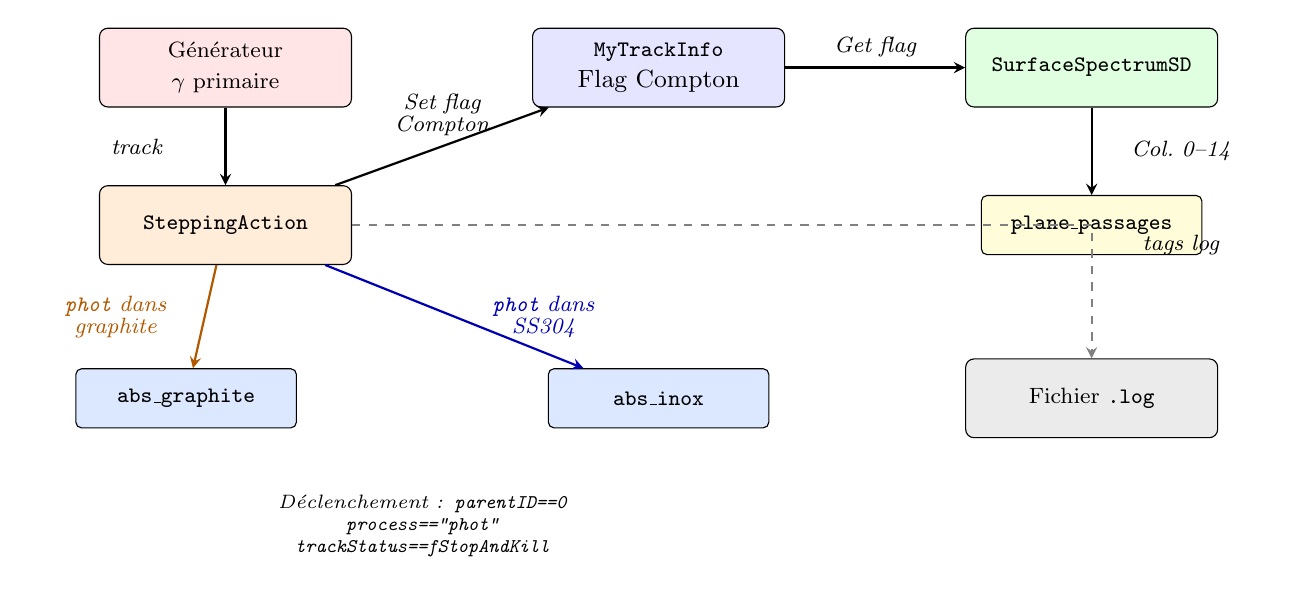
\begin{tikzpicture}[
  box/.style={draw, rounded corners=3pt, minimum height=1cm, minimum width=3.2cm,
              text centered, font=\small, align=center},
  ntuple/.style={draw, rounded corners=2pt, minimum height=0.75cm, minimum width=2.8cm,
              text centered, font=\small\ttfamily, fill=yellow!15, align=center},
  arrow/.style={->, >=stealth, thick},
  note/.style={font=\scriptsize\itshape, text=black, align=center, text width=2cm},
]

% Source
\node[box, fill=red!10] (gen) at (0, 2) {\footnotesize G\'en\'erateur\\\footnotesize $\gamma$ primaire};

% SteppingAction
\node[box, fill=orange!15] (step) at (0, 0) {\footnotesize \texttt{SteppingAction}};

% MyTrackInfo
\node[box, fill=blue!10] (info) at (5.5, 2) {\footnotesize \texttt{MyTrackInfo}\\Flag Compton};

% SurfaceSpectrumSD
\node[box, fill=green!12] (sd) at (11, 2) {\footnotesize \texttt{SurfaceSpectrumSD}};

% Ntuples
\node[ntuple] (nt_plane) at (11, 0) {\footnotesize plane\_passages};
\node[ntuple, fill=inox] (nt_graph) at (-0.5, -2.2) {\footnotesize abs\_graphite};
\node[ntuple, fill=inox]     (nt_inox)  at (5.5, -2.2) {\footnotesize abs\_inox};

% Log
\node[box, fill=black!8] (log) at (11, -2.2) {\footnotesize Fichier \texttt{.log}};

% Flèches
\draw[arrow] (gen) -- node[left, note] {\footnotesize track} (step);
\draw[arrow] (step) -- node[above, note] {\footnotesize Set flag Compton} (info);
\draw[arrow] (info) -- node[above, note] {\footnotesize Get flag} (sd);
\draw[arrow] (sd) -- node[right, note] {\footnotesize Col.\ 0--14} (nt_plane);

\draw[arrow, color=orange!70!black] (step) -- node[left, note, text=orange!70!black] {\footnotesize \texttt{phot} dans\\graphite} (nt_graph);
\draw[arrow, color=blue!70!black] (step) -- node[right, note, text=blue!70!black] {\footnotesize \texttt{phot} dans\\SS304} (nt_inox);

\draw[arrow, dashed, gray] (step) -| node[below right, note] {\footnotesize tags log} (log);

% Condition
\node[note, anchor=north, text width=5cm, align=center] at (2.5, -3.3)
  {D\'eclenchement : \texttt{parentID==0}\\
   \texttt{process=="phot"}\\
   \texttt{trackStatus==fStopAndKill}};

\end{tikzpicture}
\end{center}

%===============================================================================
\normalsize
\noindent \begin{mdframed}[backgroundcolor=orange!20]
\subsection{\color{blue}\textbf{Nouveaux tags dans le fichier \texttt{.log}}\color{black}}
\end{mdframed}
\footnotesize
%===============================================================================
% ===================================================================
%  TAGS LOG
% ===================================================================

\begin{table}[H]
\centering
\captionsetup{labelformat=empty}
\caption{\footnotesize \textit{Tags de log ajout\'es pour le suivi des photoabsorptions}.}
\renewcommand{\arraystretch}{1.2}
{\small
\begin{tabular}{llll}
\toprule
\footnotesize \textbf{Tag}&\footnotesize \textbf{Source}&\footnotesize \textbf{Fr\'equence}&\footnotesize \textbf{Contenu} \\
\midrule
\scriptsize \texttt{[STEP][ABS\_GRAPHITE]}
  &\footnotesize \texttt{SteppingAction}
  &\footnotesize 50 premiers, puis 1/10\,000
  &\footnotesize \'Ev\'enement, $E$, position, flag Compton \\[4pt]
\scriptsize \texttt{[STEP][ABS\_INOX]}
  &\footnotesize \texttt{SteppingAction}
  &\footnotesize 50 premiers, puis 1/10\,000
  &\footnotesize \'Ev\'enement, $E$, volume, position, flag Compton \\
\bottomrule
\end{tabular}
}
\end{table}


%===============================================================================
\normalsize
\noindent \begin{mdframed}[backgroundcolor=orange!20]
\subsection{\color{blue}\textbf{Exemples d'analyse ROOT}\color{black}}
\end{mdframed}
\footnotesize
%===============================================================================
\medskip
% ===================================================================
%  EXEMPLES D'ANALYSE ROOT
% ===================================================================


\medskip
%===============================================================================
\normalsize
\noindent \color{blue}\textbf{Ntuple \texttt{abs\_graphite}}\color{black}
\footnotesize
%===============================================================================
\smallskip

\begin{lstlisting}[style=root]
// Spectre en energie des gamma absorbes dans le graphite
abs_graphite->Draw("ekin_keV")

// Carte (r, z) des absorptions dans le cone
abs_graphite->Draw("z_mm:sqrt(x_mm^2+y_mm^2)",
    "", "COLZ")

// Gamma ayant fait un Compton avant d'etre absorbes
abs_graphite->Draw("ekin_keV",
    "had_compton_in_cone==1")

// Profil z des absorptions directes vs post-Compton
abs_graphite->Draw("z_mm",
    "had_compton_in_cone==0", "", "SAME")
abs_graphite->Draw("z_mm",
    "had_compton_in_cone==1", "", "SAME")
\end{lstlisting}

\medskip
%===============================================================================
\normalsize
\noindent \color{blue}\textbf{Ntuple \texttt{abs\_inox}}\color{black}
\footnotesize
%===============================================================================
\smallskip

\begin{lstlisting}[style=root]
// Spectre dans le porte-collimateur uniquement
abs_inox->Draw("ekin_keV",
    "volume==\"logicPorteCollimateur\"")

// Spectre dans l'enveloppe uniquement
abs_inox->Draw("ekin_keV",
    "volume==\"logicEnveloppeGDML\"")

// Carte (x, z) de toutes les absorptions inox
abs_inox->Draw("z_mm:x_mm", "", "COLZ")

// Comparaison porte-collimateur vs enveloppe
abs_inox->Draw("ekin_keV",
    "volume==\"logicPorteCollimateur\"")
abs_inox->Draw("ekin_keV",
    "volume==\"logicEnveloppeGDML\"", "", "SAME")

// Gamma ayant suivi un Compton avant absorption inox
abs_inox->Draw("z_mm",
    "had_compton_in_cone==1")
\end{lstlisting}

\medskip
%===============================================================================
\normalsize
\noindent \color{blue}\textbf{Analyses crois\'ees}\color{black}
\footnotesize
%===============================================================================
\smallskip

\begin{lstlisting}[style=root]
// Comptages totaux
cout << "Abs graphite : "
     << abs_graphite->GetEntries() << endl;
cout << "Abs inox     : "
     << abs_inox->GetEntries() << endl;

// Fraction des gamma ayant subi un Compton avant absorption
cout << "Graphite post-Compton : "
     << abs_graphite->GetEntries("had_compton_in_cone==1")
     << " / " << abs_graphite->GetEntries() << endl;

// Rapport avec les transmis au ScorePlane
cout << "Transmis directs     : "
     << plane_passages->GetEntries(
        "pdg==22 && is_secondary==0 && compton_in_cone==0")
     << endl;
cout << "Transmis Compton     : "
     << plane_passages->GetEntries(
        "pdg==22 && is_secondary==0 && compton_in_cone==1")
     << endl;
\end{lstlisting}


\end{document}
